
%% bare_adv.tex
%% V1.4b
%% 2015/08/26
%% by Michael Shell
%% See:
%% http://www.michaelshell.org/
%% for current contact information.
%%
%% This is a skeleton file demonstrating the advanced use of IEEEtran.cls
%% (requires IEEEtran.cls version 1.8b or later) with an IEEE Computer
%% Society journal paper.
%%
%% Support sites:
%% http://www.michaelshell.org/tex/ieeetran/
%% http://www.ctan.org/pkg/ieeetran
%% and
%% http://www.ieee.org/

%%*************************************************************************
%% Legal Notice:
%% This code is offered as-is without any warranty either expressed or
%% implied; without even the implied warranty of MERCHANTABILITY or
%% FITNESS FOR A PARTICULAR PURPOSE!
%% User assumes all risk.
%% In no event shall the IEEE or any contributor to this code be liable for
%% any damages or losses, including, but not limited to, incidental,
%% consequential, or any other damages, resulting from the use or misuse
%% of any information contained here.
%%
%% All comments are the opinions of their respective authors and are not
%% necessarily endorsed by the IEEE.
%%
%% This work is distributed under the LaTeX Project Public License (LPPL)
%% ( http://www.latex-project.org/ ) version 1.3, and may be freely used,
%% distributed and modified. A copy of the LPPL, version 1.3, is included
%% in the base LaTeX documentation of all distributions of LaTeX released
%% 2003/12/01 or later.
%% Retain all contribution notices and credits.
%% ** Modified files should be clearly indicated as such, including  **
%% ** renaming them and changing author support contact information. **
%%*************************************************************************


% *** Authors should verify (and, if needed, correct) their LaTeX system  ***
% *** with the testflow diagnostic prior to trusting their LaTeX platform ***
% *** with production work. The IEEE's font choices and paper sizes can   ***
% *** trigger bugs that do not appear when using other class files.       ***                          ***
% The testflow support page is at:
% http://www.michaelshell.org/tex/testflow/


% IEEEtran V1.7 and later provides for these CLASSINPUT macros to allow the
% user to reprogram some IEEEtran.cls defaults if needed. These settings
% override the internal defaults of IEEEtran.cls regardless of which class
% options are used. Do not use these unless you have good reason to do so as
% they can result in nonIEEE compliant documents. User beware. ;)
%
%\newcommand{\CLASSINPUTbaselinestretch}{1.0} % baselinestretch
%\newcommand{\CLASSINPUTinnersidemargin}{1in} % inner side margin
%\newcommand{\CLASSINPUToutersidemargin}{1in} % outer side margin
%\newcommand{\CLASSINPUTtoptextmargin}{1in}   % top text margin
%\newcommand{\CLASSINPUTbottomtextmargin}{1in}% bottom text margin




%
\documentclass[10pt,journal,compsoc]{IEEEtran}
% If IEEEtran.cls has not been installed into the LaTeX system files,
% manually specify the path to it like:
% \documentclass[10pt,journal,compsoc]{../sty/IEEEtran}


% For Computer Society journals, IEEEtran defaults to the use of
% Palatino/Palladio as is done in IEEE Computer Society journals.
% To go back to Times Roman, you can use this code:
%\renewcommand{\rmdefault}{ptm}\selectfont





% Some very useful LaTeX packages include:
% (uncomment the ones you want to load)



% *** MISC UTILITY PACKAGES ***
%
%\usepackage{ifpdf}
% Heiko Oberdiek's ifpdf.sty is very useful if you need conditional
% compilation based on whether the output is pdf or dvi.
% usage:
% \ifpdf
%   % pdf code
% \else
%   % dvi code
% \fi
% The latest version of ifpdf.sty can be obtained from:
% http://www.ctan.org/pkg/ifpdf
% Also, note that IEEEtran.cls V1.7 and later provides a builtin
% \ifCLASSINFOpdf conditional that works the same way.
% When switching from latex to pdflatex and vice-versa, the compiler may
% have to be run twice to clear warning/error messages.






% *** CITATION PACKAGES ***
%
\usepackage{subfigure}
\usepackage{caption}
\usepackage{graphicx}
\usepackage{booktabs}
\usepackage[space]{ctex}
\usepackage[linesnumbered,boxed,ruled,commentsnumbered]{algorithm2e}
\ifCLASSOPTIONcompsoc
  % The IEEE Computer Society needs nocompress option
  % requires cite.sty v4.0 or later (November 2003)
  \usepackage[nocompress]{cite}
\else
  % normal IEEE
  \usepackage{cite}
\fi
\usepackage{indentfirst}
% cite.sty was written by Donald Arseneau
% V1.6 and later of IEEEtran pre-defines the format of the cite.sty package
% \cite{} output to follow that of the IEEE. Loading the cite package will
% result in citation numbers being automatically sorted and properly
% "compressed/ranged". e.g., [1], [9], [2], [7], [5], [6] without using
% cite.sty will become [1], [2], [5]--[7], [9] using cite.sty. cite.sty's
% \cite will automatically add leading space, if needed. Use cite.sty's
% noadjust option (cite.sty V3.8 and later) if you want to turn this off
% such as if a citation ever needs to be enclosed in parenthesis.
% cite.sty is already installed on most LaTeX systems. Be sure and use
% version 5.0 (2009-03-20) and later if using hyperref.sty.
% The latest version can be obtained at:
% http://www.ctan.org/pkg/cite
% The documentation is contained in the cite.sty file itself.
%
% Note that some packages require special options to format as the Computer
% Society requires. In particular, Computer Society  papers do not use
% compressed citation ranges as is done in typical IEEE papers
% (e.g., [1]-[4]). Instead, they list every citation separately in order
% (e.g., [1], [2], [3], [4]). To get the latter we need to load the cite
% package with the nocompress option which is supported by cite.sty v4.0
% and later.





% *** GRAPHICS RELATED PACKAGES ***
%
\ifCLASSINFOpdf
  % \usepackage[pdftex]{graphicx}
  % declare the path(s) where your graphic files are
  % \graphicspath{{../pdf/}{../jpeg/}}
  % and their extensions so you won't have to specify these with
  % every instance of \includegraphics
  % \DeclareGraphicsExtensions{.pdf,.jpeg,.png}
\else
  % or other class option (dvipsone, dvipdf, if not using dvips). graphicx
  % will default to the driver specified in the system graphics.cfg if no
  % driver is specified.
  % \usepackage[dvips]{graphicx}
  % declare the path(s) where your graphic files are
  % \graphicspath{{../eps/}}
  % and their extensions so you won't have to specify these with
  % every instance of \includegraphics
  % \DeclareGraphicsExtensions{.eps}
\fi
% graphicx was written by David Carlisle and Sebastian Rahtz. It is
% required if you want graphics, photos, etc. graphicx.sty is already
% installed on most LaTeX systems. The latest version and documentation
% can be obtained at:
% http://www.ctan.org/pkg/graphicx
% Another good source of documentation is "Using Imported Graphics in
% LaTeX2e" by Keith Reckdahl which can be found at:
% http://www.ctan.org/pkg/epslatex
%
% latex, and pdflatex in dvi mode, support graphics in encapsulated
% postscript (.eps) format. pdflatex in pdf mode supports graphics
% in .pdf, .jpeg, .png and .mps (metapost) formats. Users should ensure
% that all non-photo figures use a vector format (.eps, .pdf, .mps) and
% not a bitmapped formats (.jpeg, .png). The IEEE frowns on bitmapped formats
% which can result in "jaggedy"/blurry rendering of lines and letters as
% well as large increases in file sizes.
%
% You can find documentation about the pdfTeX application at:
% http://www.tug.org/applications/pdftex





% *** MATH PACKAGES ***
%
%\usepackage{amsmath}
% A popular package from the American Mathematical Society that provides
% many useful and powerful commands for dealing with mathematics.
%
% Note that the amsmath package sets \interdisplaylinepenalty to 10000
% thus preventing page breaks from occurring within multiline equations. Use:
%\interdisplaylinepenalty=2500
% after loading amsmath to restore such page breaks as IEEEtran.cls normally
% does. amsmath.sty is already installed on most LaTeX systems. The latest
% version and documentation can be obtained at:
% http://www.ctan.org/pkg/amsmath





% *** SPECIALIZED LIST PACKAGES ***
%\usepackage{acronym}
% acronym.sty was written by Tobias Oetiker. This package provides tools for
% managing documents with large numbers of acronyms. (You don't *have* to
% use this package - unless you have a lot of acronyms, you may feel that
% such package management of them is bit of an overkill.)
% Do note that the acronym environment (which lists acronyms) will have a
% problem when used under IEEEtran.cls because acronym.sty relies on the
% description list environment - which IEEEtran.cls has customized for
% producing IEEE style lists. A workaround is to declared the longest
% label width via the IEEEtran.cls \IEEEiedlistdecl global control:
%
% \renewcommand{\IEEEiedlistdecl}{\IEEEsetlabelwidth{SONET}}
% \begin{acronym}
%
% \end{acronym}
% \renewcommand{\IEEEiedlistdecl}{\relax}% remember to reset \IEEEiedlistdecl
%
% instead of using the acronym environment's optional argument.
% The latest version and documentation can be obtained at:
% http://www.ctan.org/pkg/acronym


%\usepackage{algorithmic}
% algorithmic.sty was written by Peter Williams and Rogerio Brito.
% This package provides an algorithmic environment fo describing algorithms.
% You can use the algorithmic environment in-text or within a figure
% environment to provide for a floating algorithm. Do NOT use the algorithm
% floating environment provided by algorithm.sty (by the same authors) or
% algorithm2e.sty (by Christophe Fiorio) as the IEEE does not use dedicated
% algorithm float types and packages that provide these will not provide
% correct IEEE style captions. The latest version and documentation of
% algorithmic.sty can be obtained at:
% http://www.ctan.org/pkg/algorithms
% Also of interest may be the (relatively newer and more customizable)
% algorithmicx.sty package by Szasz Janos:
% http://www.ctan.org/pkg/algorithmicx




% *** ALIGNMENT PACKAGES ***
%
%\usepackage{array}
% Frank Mittelbach's and David Carlisle's array.sty patches and improves
% the standard LaTeX2e array and tabular environments to provide better
% appearance and additional user controls. As the default LaTeX2e table
% generation code is lacking to the point of almost being broken with
% respect to the quality of the end results, all users are strongly
% advised to use an enhanced (at the very least that provided by array.sty)
% set of table tools. array.sty is already installed on most systems. The
% latest version and documentation can be obtained at:
% http://www.ctan.org/pkg/array


%\usepackage{mdwmath}
%\usepackage{mdwtab}
% Also highly recommended is Mark Wooding's extremely powerful MDW tools,
% especially mdwmath.sty and mdwtab.sty which are used to format equations
% and tables, respectively. The MDWtools set is already installed on most
% LaTeX systems. The lastest version and documentation is available at:
% http://www.ctan.org/pkg/mdwtools


% IEEEtran contains the IEEEeqnarray family of commands that can be used to
% generate multiline equations as well as matrices, tables, etc., of high
% quality.


%\usepackage{eqparbox}
% Also of notable interest is Scott Pakin's eqparbox package for creating
% (automatically sized) equal width boxes - aka "natural width parboxes".
% Available at:
% http://www.ctan.org/pkg/eqparbox




% *** SUBFIGURE PACKAGES ***
%\ifCLASSOPTIONcompsoc
%  \usepackage[caption=false,font=footnotesize,labelfont=sf,textfont=sf]{subfig}
%\else
%  \usepackage[caption=false,font=footnotesize]{subfig}
%\fi
% subfig.sty, written by Steven Douglas Cochran, is the modern replacement
% for subfigure.sty, the latter of which is no longer maintained and is
% incompatible with some LaTeX packages including fixltx2e. However,
% subfig.sty requires and automatically loads Axel Sommerfeldt's caption.sty
% which will override IEEEtran.cls' handling of captions and this will result
% in non-IEEE style figure/table captions. To prevent this problem, be sure
% and invoke subfig.sty's "caption=false" package option (available since
% subfig.sty version 1.3, 2005/06/28) as this is will preserve IEEEtran.cls
% handling of captions.
% Note that the Computer Society format requires a sans serif font rather
% than the serif font used in traditional IEEE formatting and thus the need
% to invoke different subfig.sty package options depending on whether
% compsoc mode has been enabled.
%
% The latest version and documentation of subfig.sty can be obtained at:
% http://www.ctan.org/pkg/subfig




% *** FLOAT PACKAGES ***
%
%\usepackage{fixltx2e}
% fixltx2e, the successor to the earlier fix2col.sty, was written by
% Frank Mittelbach and David Carlisle. This package corrects a few problems
% in the LaTeX2e kernel, the most notable of which is that in current
% LaTeX2e releases, the ordering of single and double column floats is not
% guaranteed to be preserved. Thus, an unpatched LaTeX2e can allow a
% single column figure to be placed prior to an earlier double column
% figure.
% Be aware that LaTeX2e kernels dated 2015 and later have fixltx2e.sty's
% corrections already built into the system in which case a warning will
% be issued if an attempt is made to load fixltx2e.sty as it is no longer
% needed.
% The latest version and documentation can be found at:
% http://www.ctan.org/pkg/fixltx2e


%\usepackage{stfloats}
% stfloats.sty was written by Sigitas Tolusis. This package gives LaTeX2e
% the ability to do double column floats at the bottom of the page as well
% as the top. (e.g., "\begin{figure*}[!b]" is not normally possible in
% LaTeX2e). It also provides a command:
%\fnbelowfloat
% to enable the placement of footnotes below bottom floats (the standard
% LaTeX2e kernel puts them above bottom floats). This is an invasive package
% which rewrites many portions of the LaTeX2e float routines. It may not work
% with other packages that modify the LaTeX2e float routines. The latest
% version and documentation can be obtained at:
% http://www.ctan.org/pkg/stfloats
% Do not use the stfloats baselinefloat ability as the IEEE does not allow
% \baselineskip to stretch. Authors submitting work to the IEEE should note
% that the IEEE rarely uses double column equations and that authors should try
% to avoid such use. Do not be tempted to use the cuted.sty or midfloat.sty
% packages (also by Sigitas Tolusis) as the IEEE does not format its papers in
% such ways.
% Do not attempt to use stfloats with fixltx2e as they are incompatible.
% Instead, use Morten Hogholm'a dblfloatfix which combines the features
% of both fixltx2e and stfloats:
%
% \usepackage{dblfloatfix}
% The latest version can be found at:
% http://www.ctan.org/pkg/dblfloatfix


%\ifCLASSOPTIONcaptionsoff
%  \usepackage[nomarkers]{endfloat}
% \let\MYoriglatexcaption\caption
% \renewcommand{\caption}[2][\relax]{\MYoriglatexcaption[#2]{#2}}
%\fi
% endfloat.sty was written by James Darrell McCauley, Jeff Goldberg and
% Axel Sommerfeldt. This package may be useful when used in conjunction with
% IEEEtran.cls'  captionsoff option. Some IEEE journals/societies require that
% submissions have lists of figures/tables at the end of the paper and that
% figures/tables without any captions are placed on a page by themselves at
% the end of the document. If needed, the draftcls IEEEtran class option or
% \CLASSINPUTbaselinestretch interface can be used to increase the line
% spacing as well. Be sure and use the nomarkers option of endfloat to
% prevent endfloat from "marking" where the figures would have been placed
% in the text. The two hack lines of code above are a slight modification of
% that suggested by in the endfloat docs (section 8.4.1) to ensure that
% the full captions always appear in the list of figures/tables - even if
% the user used the short optional argument of \caption[]{}.
% IEEE papers do not typically make use of \caption[]'s optional argument,
% so this should not be an issue. A similar trick can be used to disable
% captions of packages such as subfig.sty that lack options to turn off
% the subcaptions:
% For subfig.sty:
% \let\MYorigsubfloat\subfloat
% \renewcommand{\subfloat}[2][\relax]{\MYorigsubfloat[]{#2}}
% However, the above trick will not work if both optional arguments of
% the \subfloat command are used. Furthermore, there needs to be a
% description of each subfigure *somewhere* and endfloat does not add
% subfigure captions to its list of figures. Thus, the best approach is to
% avoid the use of subfigure captions (many IEEE journals avoid them anyway)
% and instead reference/explain all the subfigures within the main caption.
% The latest version of endfloat.sty and its documentation can obtained at:
% http://www.ctan.org/pkg/endfloat
%
% The IEEEtran \ifCLASSOPTIONcaptionsoff conditional can also be used
% later in the document, say, to conditionally put the References on a
% page by themselves.





% *** PDF, URL AND HYPERLINK PACKAGES ***
%
%\usepackage{url}
% url.sty was written by Donald Arseneau. It provides better support for
% handling and breaking URLs. url.sty is already installed on most LaTeX
% systems. The latest version and documentation can be obtained at:
% http://www.ctan.org/pkg/url
% Basically, \url{my_url_here}.


% NOTE: PDF thumbnail features are not required in IEEE papers
%       and their use requires extra complexity and work.
%\ifCLASSINFOpdf
%  \usepackage[pdftex]{thumbpdf}
%\else
%  \usepackage[dvips]{thumbpdf}
%\fi
% thumbpdf.sty and its companion Perl utility were written by Heiko Oberdiek.
% It allows the user a way to produce PDF documents that contain fancy
% thumbnail images of each of the pages (which tools like acrobat reader can
% utilize). This is possible even when using dvi->ps->pdf workflow if the
% correct thumbpdf driver options are used. thumbpdf.sty incorporates the
% file containing the PDF thumbnail information (filename.tpm is used with
% dvips, filename.tpt is used with pdftex, where filename is the base name of
% your tex document) into the final ps or pdf output document. An external
% utility, the thumbpdf *Perl script* is needed to make these .tpm or .tpt
% thumbnail files from a .ps or .pdf version of the document (which obviously
% does not yet contain pdf thumbnails). Thus, one does a:
%
% thumbpdf filename.pdf
%
% to make a filename.tpt, and:
%
% thumbpdf --mode dvips filename.ps
%
% to make a filename.tpm which will then be loaded into the document by
% thumbpdf.sty the NEXT time the document is compiled (by pdflatex or
% latex->dvips->ps2pdf). Users must be careful to regenerate the .tpt and/or
% .tpm files if the main document changes and then to recompile the
% document to incorporate the revised thumbnails to ensure that thumbnails
% match the actual pages. It is easy to forget to do this!
%
% Unix systems come with a Perl interpreter. However, MS Windows users
% will usually have to install a Perl interpreter so that the thumbpdf
% script can be run. The Ghostscript PS/PDF interpreter is also required.
% See the thumbpdf docs for details. The latest version and documentation
% can be obtained at.
% http://www.ctan.org/pkg/thumbpdf


% NOTE: PDF hyperlink and bookmark features are not required in IEEE
%       papers and their use requires extra complexity and work.
% *** IF USING HYPERREF BE SURE AND CHANGE THE EXAMPLE PDF ***
% *** TITLE/SUBJECT/AUTHOR/KEYWORDS INFO BELOW!!           ***
\newcommand\MYhyperrefoptions{bookmarks=true,bookmarksnumbered=true,
pdfpagemode={UseOutlines},plainpages=false,pdfpagelabels=true,
colorlinks=true,linkcolor={black},citecolor={black},urlcolor={black},
pdftitle={Bare Demo of IEEEtran.cls for Computer Society Journals},%<!CHANGE!
pdfsubject={Typesetting},%<!CHANGE!
pdfauthor={Michael D. Shell},%<!CHANGE!
pdfkeywords={Computer Society, IEEEtran, journal, LaTeX, paper,
             template}}%<^!CHANGE!
%\ifCLASSINFOpdf
%\usepackage[\MYhyperrefoptions,pdftex]{hyperref}
%\else
%\usepackage[\MYhyperrefoptions,breaklinks=true,dvips]{hyperref}
%\usepackage{breakurl}
%\fi
% One significant drawback of using hyperref under DVI output is that the
% LaTeX compiler cannot break URLs across lines or pages as can be done
% under pdfLaTeX's PDF output via the hyperref pdftex driver. This is
% probably the single most important capability distinction between the
% DVI and PDF output. Perhaps surprisingly, all the other PDF features
% (PDF bookmarks, thumbnails, etc.) can be preserved in
% .tex->.dvi->.ps->.pdf workflow if the respective packages/scripts are
% loaded/invoked with the correct driver options (dvips, etc.).
% As most IEEE papers use URLs sparingly (mainly in the references), this
% may not be as big an issue as with other publications.
%
% That said, Vilar Camara Neto created his breakurl.sty package which
% permits hyperref to easily break URLs even in dvi mode.
% Note that breakurl, unlike most other packages, must be loaded
% AFTER hyperref. The latest version of breakurl and its documentation can
% be obtained at:
% http://www.ctan.org/pkg/breakurl
% breakurl.sty is not for use under pdflatex pdf mode.
%
% The advanced features offer by hyperref.sty are not required for IEEE
% submission, so users should weigh these features against the added
% complexity of use.
% The package options above demonstrate how to enable PDF bookmarks
% (a type of table of contents viewable in Acrobat Reader) as well as
% PDF document information (title, subject, author and keywords) that is
% viewable in Acrobat reader's Document_Properties menu. PDF document
% information is also used extensively to automate the cataloging of PDF
% documents. The above set of options ensures that hyperlinks will not be
% colored in the text and thus will not be visible in the printed page,
% but will be active on "mouse over". USING COLORS OR OTHER HIGHLIGHTING
% OF HYPERLINKS CAN RESULT IN DOCUMENT REJECTION BY THE IEEE, especially if
% these appear on the "printed" page. IF IN DOUBT, ASK THE RELEVANT
% SUBMISSION EDITOR. You may need to add the option hypertexnames=false if
% you used duplicate equation numbers, etc., but this should not be needed
% in normal IEEE work.
% The latest version of hyperref and its documentation can be obtained at:
% http://www.ctan.org/pkg/hyperref





% *** Do not adjust lengths that control margins, column widths, etc. ***
% *** Do not use packages that alter fonts (such as pslatex).         ***
% There should be no need to do such things with IEEEtran.cls V1.6 and later.
% (Unless specifically asked to do so by the journal or conference you plan
% to submit to, of course. )
\renewcommand\tablename{table}

% correct bad hyphenation here
\hyphenation{op-tical net-works semi-conduc-tor}


\begin{document}
\captionsetup{font={scriptsize}}
%
% paper title
% Titles are generally capitalized except for words such as a, an, and, as,
% at, but, by, for, in, nor, of, on, or, the, to and up, which are usually
% not capitalized unless they are the first or last word of the title.
% Linebreaks \\ can be used within to get better formatting as desired.
% Do not put math or special symbols in the title.
\title{Visualization of Flow Field based on Centroidal Voronoi Tessellation}
%
%
% author names and IEEE memberships
% note positions of commas and nonbreaking spaces ( ~ ) LaTeX will not break
% a structure at a ~ so this keeps an author's name from being broken across
% two lines.
% use \thanks{} to gain access to the first footnote area
% a separate \thanks must be used for each paragraph as LaTeX2e's \thanks
% was not built to handle multiple paragraphs
%
%
%\IEEEcompsocitemizethanks is a special \thanks that produces the bulleted
% lists the Computer Society journals use for "first footnote" author
% affiliations. Use \IEEEcompsocthanksitem which works much like \item
% for each affiliation group. When not in compsoc mode,
% \IEEEcompsocitemizethanks becomes like \thanks and
% \IEEEcompsocthanksitem becomes a line break with idention. This
% facilitates dual compilation, although admittedly the differences in the
% desired content of \author between the different types of papers makes a
% one-size-fits-all approach a daunting prospect. For instance, compsoc
% journal papers have the author affiliations above the "Manuscript
% received ..."  text while in non-compsoc journals this is reversed. Sigh.

\author{Michael~Shell,~\IEEEmembership{Member,~IEEE,}
        John~Doe,~\IEEEmembership{Fellow,~OSA,}
        and~Jane~Doe,~\IEEEmembership{Life~Fellow,~IEEE}% <-this % stops a space
\IEEEcompsocitemizethanks{\IEEEcompsocthanksitem M. Shell was with the Department
of Electrical and Computer Engineering, Georgia Institute of Technology, Atlanta,
GA, 30332.\protect\\
% note need leading \protect in front of \\ to get a newline within \thanks as
% \\ is fragile and will error, could use \hfil\break instead.
E-mail: see http://www.michaelshell.org/contact.html
\IEEEcompsocthanksitem J. Doe and J. Doe are with Anonymous University.}% <-this % stops a space
\thanks{Manuscript received April 19, 2005; revised August 26, 2015.}}

% note the % following the last \IEEEmembership and also \thanks -
% these prevent an unwanted space from occurring between the last author name
% and the end of the author line. i.e., if you had this:
%
% \author{....lastname \thanks{...} \thanks{...} }
%                     ^------------^------------^----Do not want these spaces!
%
% a space would be appended to the last name and could cause every name on that
% line to be shifted left slightly. This is one of those "LaTeX things". For
% instance, "\textbf{A} \textbf{B}" will typeset as "A B" not "AB". To get
% "AB" then you have to do: "\textbf{A}\textbf{B}"
% \thanks is no different in this regard, so shield the last } of each \thanks
% that ends a line with a % and do not let a space in before the next \thanks.
% Spaces after \IEEEmembership other than the last one are OK (and needed) as
% you are supposed to have spaces between the names. For what it is worth,
% this is a minor point as most people would not even notice if the said evil
% space somehow managed to creep in.



% The paper headers
\markboth{Journal of \LaTeX\ Class Files,~Vol.~14, No.~8, August~2015}%
{Shell \MakeLowercase{\textit{et al.}}: Bare Advanced Demo of IEEEtran.cls for IEEE Computer Society Journals}
% The only time the second header will appear is for the odd numbered pages
% after the title page when using the twoside option.
%
% *** Note that you probably will NOT want to include the author's ***
% *** name in the headers of peer review papers.                   ***
% You can use \ifCLASSOPTIONpeerreview for conditional compilation here if
% you desire.



% The publisher's ID mark at the bottom of the page is less important with
% Computer Society journal papers as those publications place the marks
% outside of the main text columns and, therefore, unlike regular IEEE
% journals, the available text space is not reduced by their presence.
% If you want to put a publisher's ID mark on the page you can do it like
% this:
%\IEEEpubid{0000--0000/00\$00.00~\copyright~2015 IEEE}
% or like this to get the Computer Society new two part style.
%\IEEEpubid{\makebox[\columnwidth]{\hfill 0000--0000/00/\$00.00~\copyright~2015 IEEE}%
%\hspace{\columnsep}\makebox[\columnwidth]{Published by the IEEE Computer Society\hfill}}
% Remember, if you use this you must call \IEEEpubidadjcol in the second
% column for its text to clear the IEEEpubid mark (Computer Society journal
% papers don't need this extra clearance.)



% use for special paper notices
%\IEEEspecialpapernotice{(Invited Paper)}



% for Computer Society papers, we must declare the abstract and index terms
% PRIOR to the title within the \IEEEtitleabstractindextext IEEEtran
% command as these need to go into the title area created by \maketitle.
% As a general rule, do not put math, special symbols or citations
% in the abstract or keywords.
\IEEEtitleabstractindextext{%
\begin{abstract}
\indent A Centroidal Voronoi Tessellation (CVT) is a Voronoi Tessellation in which the generators are the centroids for each Voronoi region.By this kind of tessellation,the centroids represent the whole region's information.It is likely to convey us some characteristics while the common Voronoi Tessellation can't.Meanwhile,Visualization in Scientific Computing(ViSC) just requires us visualizing the representative characteristics of the field.In this case, it can be done with a few points or arrows to express a lot of information,by combining the CVT with the flow field visualization, and generating the image that can be more accessible to people.\\
\indent In this paper,it is mentioned that what is ViSC and CVTs.Then focusing on how to generate a CVT and how to use CVT to generate a characteristic visualization,for steady field as well as consecutive field.
\end{abstract}

% Note that keywords are not normally used for peerreview papers.
\begin{IEEEkeywords}
Scientific Visualization,Visualization in Scientific Computing,Centroidal Voronoi tessellation,Flow Field
\end{IEEEkeywords}}


% make the title area
\maketitle


% To allow for easy dual compilation without having to reenter the
% abstract/keywords data, the \IEEEtitleabstractindextext text will
% not be used in maketitle, but will appear (i.e., to be "transported")
% here as \IEEEdisplaynontitleabstractindextext when compsoc mode
% is not selected <OR> if conference mode is selected - because compsoc
% conference papers position the abstract like regular (non-compsoc)
% papers do!
\IEEEdisplaynontitleabstractindextext
% \IEEEdisplaynontitleabstractindextext has no effect when using
% compsoc under a non-conference mode.


% For peer review papers, you can put extra information on the cover
% page as needed:
% \ifCLASSOPTIONpeerreview
% \begin{center} \bfseries EDICS Category: 3-BBND \end{center}
% \fi
%
% For peerreview papers, this IEEEtran command inserts a page break and
% creates the second title. It will be ignored for other modes.
\IEEEpeerreviewmaketitle


\ifCLASSOPTIONcompsoc
\IEEEraisesectionheading{\section{introdution}\ }
\else
\section{}
\label{sec:introduction}
\fi
% Computer Society journal (but not conference!) papers do something unusual
% with the very first section heading (almost always called "Introduction").
% They place it ABOVE the main text! IEEEtran.cls does not automatically do
% this for you, but you can achieve this effect with the provided
% \IEEEraisesectionheading{} command. Note the need to keep any \label that
% is to refer to the section immediately after \section in the above as
% \IEEEraisesectionheading puts \section within a raised box.




% The very first letter is a 2 line initial drop letter followed
% by the rest of the first word in caps (small caps for compsoc).
%
% form to use if the first word consists of a single letter:
% \IEEEPARstart{A}{demo} file is ....
%
% form to use if you need the single drop letter followed by
% normal text (unknown if ever used by the IEEE):
% \IEEEPARstart{A}{}demo file is ....
%
% Some journals put the first two words in caps:
% \IEEEPARstart{T}{his demo} file is ....
%
% Here we have the typical use of a "T" for an initial drop letter
% and "HIS" in caps to complete the first word.
\indent Visualization in Scientific Computing, witch refers to the action of converting from the scientific computing and experimental data to the images that accessible to commons.Since we human hardly directly comprehend and analysis big amount of data, it is necessary to convert the data before.And because visual information accounted for the vast majority of all the information which human obtains, it will be more conveniently and successfully to convert the data to the image helping people comprehend the data briefly.So that scientists can get the general impression of the data which leads the direction for further research. However,due to the structure of human eye,it is hardly to distinguish the difference of images in detail.So that simply rendering every data to generate an image may cover the details which sometimes can be the information we desire.At this point,it is better to extract the characteristics of the data and then only visualizing the characteristic information.That is the reason why we steadily developing the algorithm of ViSC,both on the higher computing speed and better characteristic extraction.\\
\indent In this section, the brief development history of ViSC would be shown. So that we can have a deeper understand of why and how we do the ViSC.



\subsection{History and Background of Visualization}
\indent Visualization, as the name implies, is to convert the non-graphical objects to graphical things, non-visual information into visual information.
\indent In fact, the earliest visualization can pursue to the very old.For a simple example, from the abstract number "2" to the symbol "$\romannumeral2 $", is a kind of visualization.Although $\romannumeral2 $ is still an abstract symbol , the transformation change the invisible to visible,which make the communication possible.\\
\indent Modern classification of visualization is mainly according to its processing object.It is divided into three main categories:Visualization in Scientific Computing:Visualize the data obtained from scientific computing.Information Visualization:Trans the known information,like the trading volume of stock market, into an intuitively identify graphics. Knowledge Visualization :Facilitate the communication between people by converting the knowledge or idea into graphics.As well as help human get right knowledge,just like the venn diagram.\\
\indent The word 'Visualization' was first regarded as a subject term in Feb 1987 at the symposium on graphic and images holding by NSF.Durning the symposium,the definition and the field of ViSC was established.From then on,'visualization' has became a recognized subject. \\
\indent However,due to the limit of hardware,scientific computing only processed in batch mode,during the early development of ViSC.Furthermore,without the function of interaction, it was hardly for scientists to influence or operate the process during computing.Therefore, scientists had nothing to do but waiting for the result.Meanwhile, the great amount of output was visualized manually.As the best method displaying the result in two-dimensional by an auxiliary plotter at that time, scientists spent plenty of time but obtaining the graphics with tons of information lost during the manually process.This circumstances last for years.Not until the booming development of computer graphics processing, ViSC comes into practical using.\\
% needed in second column of first page if using \IEEEpubid
%\IEEEpubidadjcol
\subsection{Present Situation of Visualization in Scientific Computing}
\indent VISC is defined as:The theory, method and technology about converting data and calculation results which are generated from scientific computing, into graphics or images to be displayed on the screen,with computer graphics and image processing technology.It relates to computer graphics, image processing, computer vision, computer aided design and graphic user interface (GUI) multiple research field.\\
\indent The purpose of visualization in scientific computing is to understand the essence of nature.To achieve this objective, the scientists convert the scientific data, including data obtained by measurements and the information obtained through scientific computing,into intuitive, graphic physical phenomena or quantities that varying with time and space and presenting in front of the researchers, so that researchers can observe, simulation and calculation.This process can be refined into the following four steps:a. filtering, preprocessing the original data, the conversion of data form, filter out noise, extract the data of interest, etc.b. mapping, the filtered data is mapped to the geometric elements, a common point, line, face graphics, 3D graphics, etc.c. rendering,drawing geometric elements , get the results of the image.d. feedback, display images, and analysis of the visual results obtained.ViSC technology is of great significance, since it greatly speeds up the processing of the data as well as enables the communication between people and machine,which enhances the ability of people observing the law of nature.So that when scientists get the results of the calculation,they will know what happened in the calculation process.Furthermore,thanks to the ViSC that scientists can change the parameters to observe its impact on the calculation process to achieve the guidance and control.\\
\indent Flow visualization is a branch of ViSC,as well as an important part of fluid mechanics.It is the research of flow field visualization that makes the calculation flow dynamics (CFD) develop rapidly.Vector and tensor fields are the main types of data in computational fluid dynamics.Flow field visualization using arrows, flow lines and particle tracking techniques to show the two-dimensional flow field.As for the three dimensional flow field, people have not found a generally accepted, intuitive visual method.Now it is mainly through the following several methods of research:a.Improving the volume rendering method.Make it able to display flow field.b. flow surface technology, using the method of flow surface and gradient to represent the flow field.c.Legend technology.d.Feature based visualization, which is carried out from the upper level to the flow field visualization.\\
\indent The CVT based visualization is belong to the forth group.It is a feature based visualization method.In this paper,we extend the CVT based visualization to several time step with small increase of time cost.So that it is able to visualize a time dependent flow field.\\
\section{Algorithms of Centroidal Voronoi tessellation}
\subsection{Centroidal Voronoi tessellation}
\indent Let us begin with the definition of the Centroidal Voronoi tessellation:\\
\indent For an point set $\Omega\subseteq\mathbf{R}^n$, denote $d(x_1,x_2)\in \mathbf{R}$ as the distance of any two points $x_1,x_2$.A tessellation,which is represented by a group of sets $\{ V_i\}^k_{i=1}$, is called Centroidal Voronoi Tessellation if it satisfies:\\
\textcircled{1}.For all the sets $V_i$ $V_i\cap V_j=\emptyset \iff i\ne j,\bigcup^k_{i=1}\overline{V_i}=\overline{\Omega}$ while $\overline{V_i},\overline{\Omega}$ is the closures of $V_i,\Omega$\\
\textcircled{2}.The centroids of all sets,denoted as $\{v_i\}_{i=1}^k$,are exactly the generators of the Voronoi Tessellation.That is:
\begin{equation}
V_i=\{x\in\Omega |d(v_i,x)<d(v_j,x),j\ne i\}
\end{equation}
\indent The centroid $v_i$ of a points set is the point $x$ that minimize the energy integration.The energy integration can be:
\begin{equation}
E(x)=\int_{V_i}\rho(s)d^2(x,s)ds
\end{equation}
\indent $\rho(s)$ refers to the density function.\\
\indent So we are able to generate voronoi tessellation through formula (1), if the generators are given.And also ,it is trivial to get the centroids of this tessellation by minimize formula (2).However,it is difficult to generate Centroidal Voronoi tessellation directly,since the centroids are generally not the generators.This implies that CVT is only a small part of all tessellation, to a certain set of point.So an effective and efficient algorithm is required,instead of solving a series of integration equations,to find the CVT.The algorithm is introduced in the next subsection.\\
\indent By the way,the distance $d$ mentioned above can be not merely Euclidean distance,but a generalized distance,which satisfy the three conditions of distance.And the density function $\rho$ can be some other function on the point set,which is 'like' the density function.This would be discussed in the later section.
\subsection{An Algorithm for Centroidal Voronoi tessellation generation}
\indent The most widely used algorithm for Centroidal Voronoi tessellation generation is a modification of Lloyd Algorithm.
\begin{algorithm}[h]
\KwIn{\\A point set $\Omega$\;\\A positive integer $k$ for dividing $\Omega$ into $k$ regions\;\\A tolerence value $\epsilon$\;}
\KwOut{\\$k$ points to be the generators of the CVT\;}

Choose any $k$ non-coincided points from $\Omega$,denote them as $\{v_i\}_{i=1}^k$.\\

\While{ture}{
For each $0<i\le k$,generate the cluster of $\{v_i\}_{i=1}^k$.Denote the clusters as $\{V_i\}_{i=1}^k$.\\
For each $0<i\le k$,determine the Centroid of $\{V_i\}_{i=1}^k$ by minimize the energy function.Denote the points as $\{\overline{v}_i\}_{i=1}^k$.\\
Calculate the variation:$\delta=\sum_{i=1}^k d(v_i,\overline{v}_i)$.\\
\eIf{$\delta\le\epsilon$}
{Output the $k$ points $\{\overline{v}_i\}_{i=1}^k$ and break the loop\;}
{Set $v_i=\overline{v}_i,i=1,\dots,k$ and continue the loop\;}
}
\caption{Lloyd Algorithm for CVT in point set}
\end{algorithm}
\\
\indent The  main idea of this algorithm is that when the aggregation of the distance between every pair of the centroidal and the generator is small,the distinct between the old and new clusters would be as small.So that we can get a group of approximative generators which would generate quite similar tessellation from the real CVT.And it is obvious that as the aggregation of distance get smaller,the distinction between the real CVT and the tessellation constructed by this algorithm will get as smaller,either.
\subsection{The Algorithm for Centroidal Vorinoi tessellation in flow field}
\indent For the a simple point set,it is enough to construct a CVT by Algorithm 1.But for a more complex set,like a flow field,more information need to be taken into consider.Once we want the centroid express the detail of the vector function, a general idea is to change the energy function.\\
\indent For an point set $\Omega\subset \mathbf{R}^n,\forall x\in \Omega$,we denote the flow field with its vector function $y=F(x)\in \mathbf{R}^m$.To minimize the energy function ,we put the following algorithm as an example:
\begin{algorithm}[h]
\caption{CVT generating algorithm for flow field}
\KwIn{\\A flow field which consists of a point set $\Omega$ and a vector function $F(x)$ on $\Omega$\;\\A positive integer $k$ for dividing $\Omega$ into $k$ regions\;\\A tolerence value $\epsilon$\;}
\KwOut{\\$k$ points to be the generators of the CVT\;\\One vector on each generator\;}
Choose $k$  points that do not coincident in $\Omega$.Denote as $\{x_i\}_{i=1}^k$\\
\While{ture}
{Generate the Vorinoi tessellation $\{V_i\}_{i=1}^k$ by the $k$ points:
  $V_i=\{x\in \Omega|d(x,x_i)<d(x,x_j),j\ne i\}$\;
Determine the centroid of each Voronoi region:
$\overline{x}_i=\frac{\int_{V_i}|F(x)|^2 xdx}{\int_{V_i}|F(x)|^2 dx}$
$\overline{y}_i=\frac{\int_{V_i}|F(x)|F(x)dx}{|\int_{V_i}|F(x)|F(x)dx|}$
$i=1,\dots ,k$\;
Calculate the variation:$\delta=\sum_{i=1}^kd(x_i,\overline{x}_i)$\;
\eIf{$\delta<\epsilon$}
{
Output the $\{\overline{x}_i,\overline{y}_i\}_{i=1}^k$ and break the loop\;
}
{
Set $\{x_i,y_i\}\{\overline{x}_i,\overline{y}_i\}_{i=1}^k$ and continue the loop\;
}
}
\end{algorithm}
\\
\indent It is supposed that the density is constant in the above algorithm.That is equivalent to $\rho(x)\equiv 1$.As for the field that has a non-constant density $\rho(x)$,we may simply change the formula into:
\begin{equation}
\overline{x}_i=\frac{\int_{V_i}\rho(x)|F(x)|^2 xdx}{\int_{V_i}\rho(x)|F(x)|^2 dx}
\end{equation}
\begin{equation}
\overline{y}_i=\frac{\int_{V_i}\rho(x)|F(x)|F(x)dx}{|\int_{V_i}\rho(x)|F(x)|F(x)dx|}
\end{equation}
for $i=1,\dots ,k$.
%\subsection{The discrete case}
%\indent Because that the practical data of fields is generally discrete points data, rather than a unified function,it is necessary to adjust the algorithm in the last subsection to the discrete case.Fortunately,it is able to simply replace the integral to summation to satisfy the discrete case.And we can get a algorithm that easier to calculate:\\
%\textbf{Algorithm 3}��For a group of discrete points data $\{c_i\}_{i=1}^n$ and the vector function $F(x)$ on the data field,choose $k$ points noncoincidence each other $\{x_i\}_{i=1}^k$\\
%��Generate the Centroid Vorinoi tessellation with the $\{x_i\}$.Divede the points $c_i$ into $k$group.Denote the groups as $V_i,i=1,2,\dots,k$.\\
%��Determine the new centroid of each group $V_i,i=1,2,\dots,k$��
%\begin{center}
%  $\overline{x}_i=\frac{\sum_{V_k}|F(x)|^2 xdx}{\sum_{V_k}|F(x)|^2 dx}\quad,\quad \overline{y}_i=\frac{\sum_{V_i}|F(x)|F(x)dx}{|\sum_{V_i}|F(x)|F(x)dx|}$
%\end{center}
%��compare the new centroid to the old generator.If the difference(the difference can be measured by the norm) between them is small enough,then end the loop.Otherwise we set $x_i=\overline{x}_i$,and return to �١�
\subsection{Several notes about the algorithm for Centroidal Voronoi tessellation}
\indent The above discussion is based on the distance definition: $d(x_1,x_2)=\sqrt{|y_1|^2-|y_1|y_1 *y_2+w|y_1|^2|x_1 -x_2|^2}$.If the distance function is changed,the energy function,the generator determination formula,and the tessellation criterion will change as well.In other word,it is a very efficient way we can choose the characteristic we expect by choose specific distance function.\\
\indent As we have known that the Lloyd Algorithm is the prototype of the algorithm introduced last two subsections.The reason why we use the Lloyd Algorithm solving this kind of k-average problem is that it converges to the solution very fast.But Lloyd algorithm can not guarantee the global optimal.However,thanks to the definition of CVT not asking for the global optimal,it is enough to generate a Centroidal Voronoi tessellation with the local optimal.\\
\indent Even though Lloyd Algorithm gets a fast rate in convergence,it would still take a long time converging to the solution when dealing with large amount of data.Further,Quasi-Newton method is used to reduce the time cost.\\
\indent Denote the union of all the generators for a voronoi tessellation as a vector $\mathbf{v}=\{v_i\}_{i=1}^k$. Then we define the total energy function as:\\
\begin{equation}
E(\mathbf{v})=\sum\limits_{i=1}^k\int_{V_i}\rho(x)(v_i-x)^2dx\\
\end{equation}
\indent It is obvious that the global optimality is as well the local optimality,and trivially leading to CVT.So minimizing the total energy function,can be an reliable method to the CVT.The algorithm is as follow:\\
\begin{algorithm}
\caption{CVT generating algorithm through minimizing total energy function}
\KwIn{\\A vector field $\Omega\in\mathbf{R}^n$ with vector function $y=F(x)$ on it\;\\
A positive integer $k$\;A threshold $\epsilon$\;}
\KwOut{\\$k$ points to be the generators of the CVT\;\\One vector on each generator}
Choose $k$ points $\mathbf{v}=\{v_i\}_{i=1}^k$\;
\While{Ture}
{
Determine the Voronoi tessellation $\{V_i\}_{i=1}^k$:
$V_i=\{x\in\Omega\vert d(v_i,x)<d{v_j,x}\}$\;
Calculate the $\partial E$ by solve the quasi-Newton function:
\begin{center}
$H\partial E=G$
\end{center}
   $H$ is the approximation Hessian of $E(\mathbf{v})$\\
   $G_i=\frac{\partial}{\partial v_i}E(\mathbf{v})=2\int_{V_i}\rho(x)(v_i-x)dx$\;
\eIf{$\Vert\partial E\Vert<\epsilon$}
{Output $\mathbf{v}$ and break the loop\;}
{Update $\mathbf{v}=\mathbf{v}+a*\partial E$\;($a$ satisfies the strong wolfe condition)}
}
\end{algorithm}
\indent Since this algorithm is based on the Quasi-Newton algorithm,it sometimes can not reach the global minimum.However,a local minimum is enough to generate a CVT.
\subsection{The CVT Algorithm for consecutive flow field***}
\indent Sometime we are aimed to visualize the flow field at several adjacent time steps,to show the change of the flow field in a certain space.And once we decide to visualize a flow field through CVT,the time that CVT generating algorithm costs is a big matter.Thanks to the contact between two adjacent time steps,it is able to save time through choosing specific initial $\{v_i\}_{i=1}^k$ in the algorithm at each time step.\\
\indent Commonly,the CVT generators at the last time step,would not be far from this time step,as long as the flow field is consecutive***.As the algorithm shows,the centroid is determined by the weighted average of all the points' position and the length of the vector at the point.In other words,as long as the vector length or the square of the vector length does not change ,the centroid' position would not change no matter how the direction of the vector changes.Similarly,if the vector length of all points in each tessellation does not change a lot,the new centroid would stay in the neighbourhood of the old one.\\
\indent Based on the above discussion,it is likely to cost less time if we choose the generators of the last CVT as the seeds.By this way,time cost can be decreased over a half comparing to the random selected seeds.And the displacement of the centroids
\begin{table}[!h]
\caption{Time cost for non-randomly selected seeds}
\begin{center}
\begin{tabular}{|c|c|c|}
  \hline
  % after \\: \hline or \cline{col1-col2} \cline{col3-col4} ...
  loop & start time(ms) & calculation finish time(ms)\\
  \hline
0 & 89 & 17834\\
5 & 51997 & 61029\\
10 & 86088 & 90436\\
15 & 121760 & 126588\\
20 & 156476 & 163923\\
25 & 195473 & 209979\\
30 & 257546 & 266173\\
35 & 310135 & 325948\\
40 & 358649 & 372275\\
45 & 417337 & 422617\\
50 & 451361 & 454023\\
55 & 459536 & 460893\\
  \hline
\end{tabular}
\end{center}
\end{table}

\begin{table}[!h]
\caption{Time cost for randomly selected seeds}
\begin{center}
\begin{tabular}{|c|c|c|}
  \hline
  % after \\: \hline or \cline{col1-col2} \cline{col3-col4} ...
  loop & start time(ms) & calculation finish time(ms)\\
  \hline
0 & 55 & 17645\\
5 & 87409 & 111617\\
10 & 176868 & 197379\\
15 & 273771 & 294030\\
20 & 370727 & 387668\\
25 & 462774 & 479188\\
30 & 551769 & 572305\\
35 & 660625 & 692617\\
40 & 780755 & 808371\\
45 & 900107 & 920976\\
50 & 1004445 & 1024704\\
55 & 1140349 & 1162175\\
  \hline
\end{tabular}
\end{center}
\end{table}































\section{Visualisation Strategies}
\indent In the last subsection,the definition and and the generating algorithm were introduced.By the Lloyd Algorithm ,CVT with the error small enough can be generated.So far,we get a group of unit vectors at the centroid of each cluster.Then it is the visualization part.
\subsection{Length}
\indent In the last section,we get the representation vectors as unit vectors at each centroid.But if we hope to show the characteristic vector of each cluster,it is needed to modify the representation vector to the characteristic length.Here the word 'characteristic' means the character we concern about,like the longest,the shortest,or the average.Generally,it is the statistics that people likely to choose as the character.Here are some example:\\
For uniform field,we need to calculate the modify factor:
\begin{equation}
  L_i=\frac{1}{|V_i|}\int_{V_i}|F(x)|dx
\end{equation}
Or
\begin{equation}
  L_i=\frac{1}{V_i}(\int_{V_i}|F(x)|^2 dx)^{1/2}
\end{equation}
As for nonuniform field:
\begin{equation}
  L_i=\frac{(\int_{V_i}\rho(x)|F(x)|^2 dx)^{1/2}}{\int_{V_i}\rho(x)dx}
\end{equation}
\indent Then,we are able to modify the output of CVT $\overline{y}_i$ to $\overline{y}_i * L_i$.The new representation vectors $\overline{y}_i*L_i$ at each centroid $\overline{x}_i$ has the different length according to the weighted average of each cluster,now.
\subsection{Color}
\indent It is generally that we use color to show the high or low.Just like the meteorogram in weather reports,bright color usually refer to high temperature and the cold color refer to low temperature.This is very common in scalar field.As for the vector field,thanks to the length of representation vectors are different that it is able to use color show other information like the density of data points,the energy calculated by the energy function,or the difference of vectors in the cluster, instead of length.We take the last one as an example.The difference of vectors in the cluster can be defined as:
\begin{equation}
  Var(V_i)=\frac{\int_{V_i}|y|^2 -|y|y\times y_i dx}{|V_i|}
\end{equation}
\indent And then normalize $Var(V_i)$ in all clusters.Use the $Var(V_i)$ as the scale of gray level or other color calibration method.So that show two characters of each cluster at same time.
\subsection{Graphic representation}
\indent As for the graphic representation,arrow and ellipse are generally used.Comparatively speaking,both has advantages and disadvantages.Arrow is good at showing direction,while ellipse takes the advantage of showing color.\\
\indent However,due to the density of points is distinct in different case,arrows or ellipses are likely to intersect each other(cross of arrows and overlap of ellipses),if the number of clusters $k$ is big and the distribution of the clusters is nonuniform.So that it is able to use short stream line locally to ensure the uncross of arrows or ellipses.Here is the algorithm:\\
\begin{algorithm}
\caption{Algorithm for short streamline generation}
\KwIn{\\Initial point $z_0$ and vector function $F(z)$\;\\Iteration times $k$\;}
\KwOut{\\A streamline\;}
\For{$i=0;i<k;i++$}{
Calculate $w_i=F(z_i)$ as the vector in this loop\;
Move $z_i$ to $z_{i+1}=z_i+\frac{w_i}{k*\vert w_i\vert}$\;
Draw a straight line from $z_i$ to $z_{i+1}$\;
}
\end{algorithm}
\par
\indent To ensure that the arrows do not across each other,it is effective to use short streamline instead of the straight arrows.To obtain short streamlines, it is able to determine the whole field through interpolation.In this way,not only the average direction of the cluster,but also the detail direction in the cluster can be demonstrated.It works well when dealing with the field with steep change in the direction,like vortex.\\
\indent With all the method discussed above,it is able to visualize what we want through CVT.By the way,when choose the figure,color,and distance,it is mostly depend on what to focus on,and the specific problem dealt with.
































\section{Applications and Numerical Example}
\indent This section mainly gives some visualization examples.\\
\indent We first concern about steady fields.In these cases,it is the characteristic that people mainly concern about,Specifically,such as vortices,extreme points,and where the gradient is quite big.To catch these key points,while not letting too much information confuse us,it is an efficient method to calculate the characteristic points by CVT.Here are two representative field visualized through CVT method:\\

\begin{center}
\begin{figure}[h]
\centering
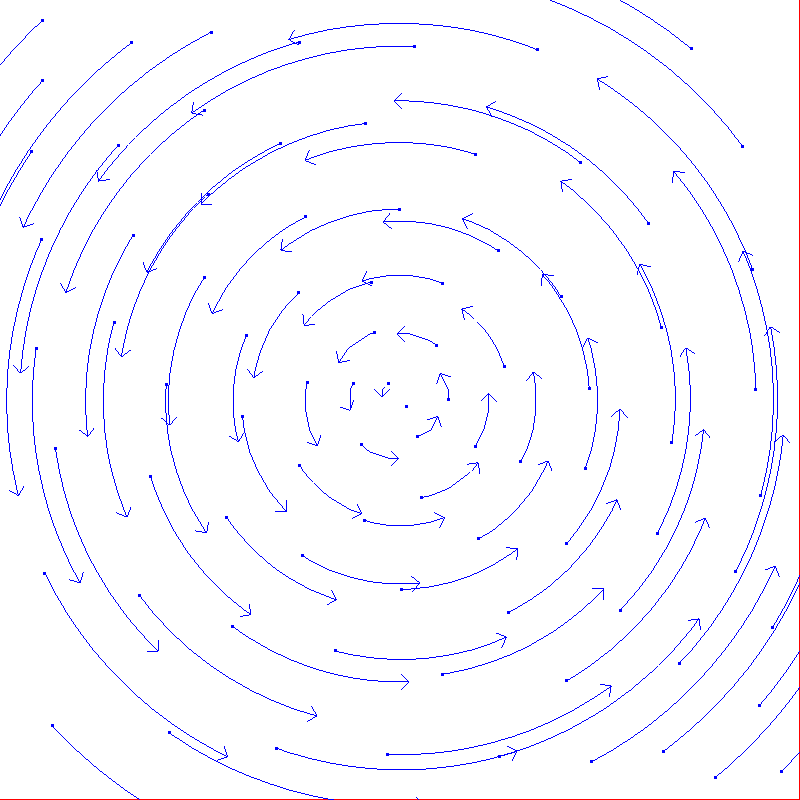
\includegraphics[width=0.3\textwidth]{cc2.png}
\caption{simple magnetic field}
\label{cc}
\end{figure}
\begin{figure}[h]
\centering
\subfigure{\label{full}}
\addtocounter{subfigure}{-2}
\subfigure[All data points drawn]{\subfigure{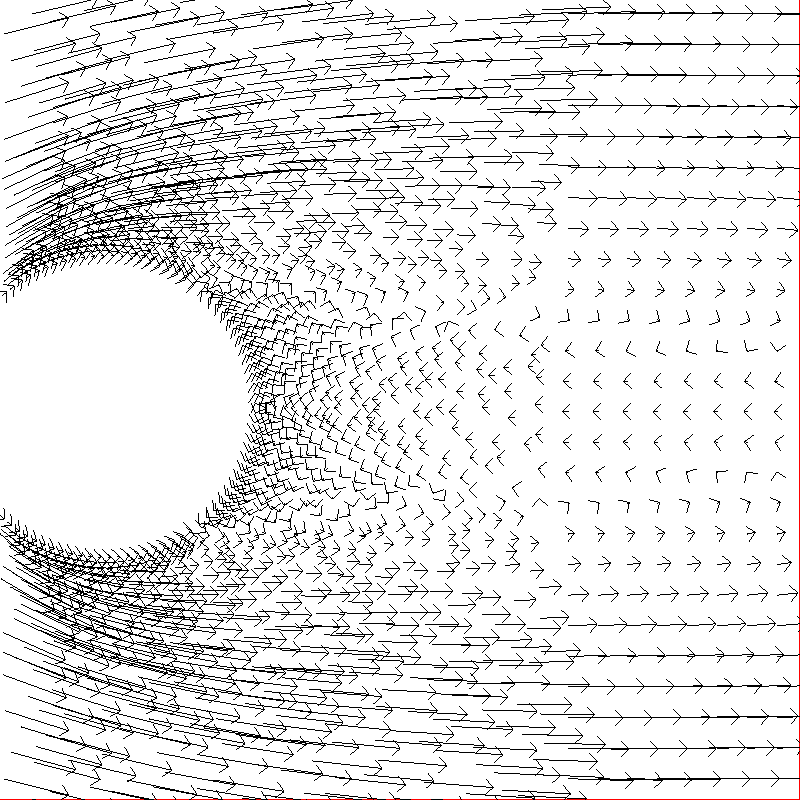
\includegraphics[width=0.2\textwidth]{full.png}}}
\subfigure{\label{CVT}}
\addtocounter{subfigure}{-2}
\subfigure[Centroids points drawn]{\subfigure{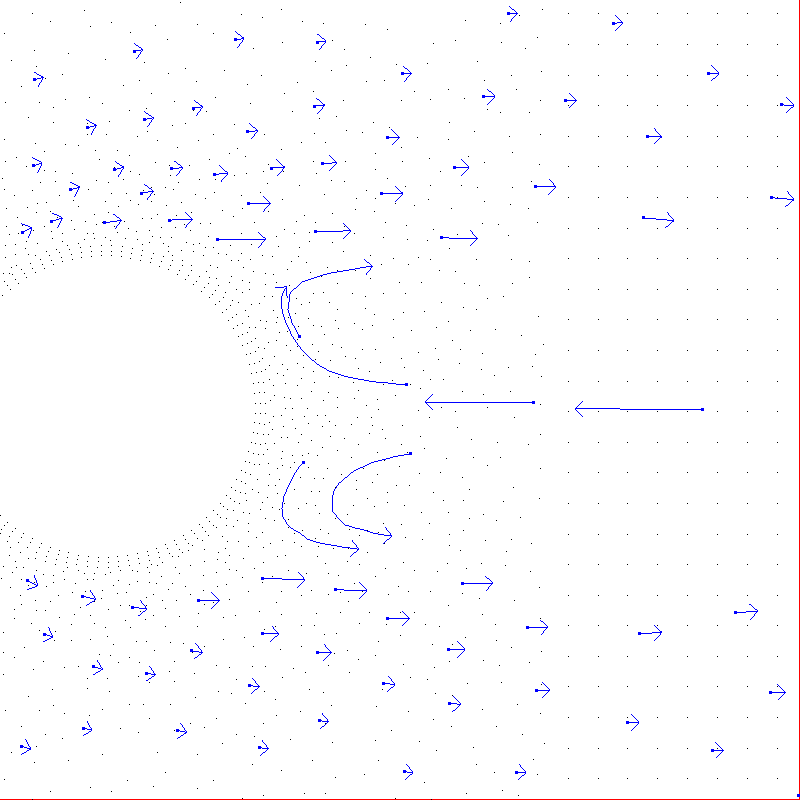
\includegraphics[width=0.2\textwidth]{CVT.png}}}
\caption{Flow around a rigid pile}
\end{figure}
\end{center}
\par
\indent In fig.\ref{cc},the characteristic of eddy is very clear,though the short streamline works bad at the center of the vortex.And in fig.\ref{full},it is the one with all data points drawn,while fig.\ref{CVT} is the one only centroids of CVT drawn.It is clear from fig.\ref{CVT} that the two vortices are laying behind the pile,while too many arrows covered this feature in fig.\ref{full}.\\
\indent As for consecutive fields,by inheriting the generators of the last step,it is able to visualize the field not only time-effective but also characteristic.Since the generators are 'tent' to gather to the points that contribute a lot in energy function,the shift of CVT generators between adjacent time steps indicates the change of the field to a certain extent.
\begin{center}
\begin{figure}[htbp]
%\centering
\begin{minipage}[t]{0.5\linewidth}
\subfigure{\label{1.1}}
\addtocounter{subfigure}{-2}
\subfigure[]{\subfigure{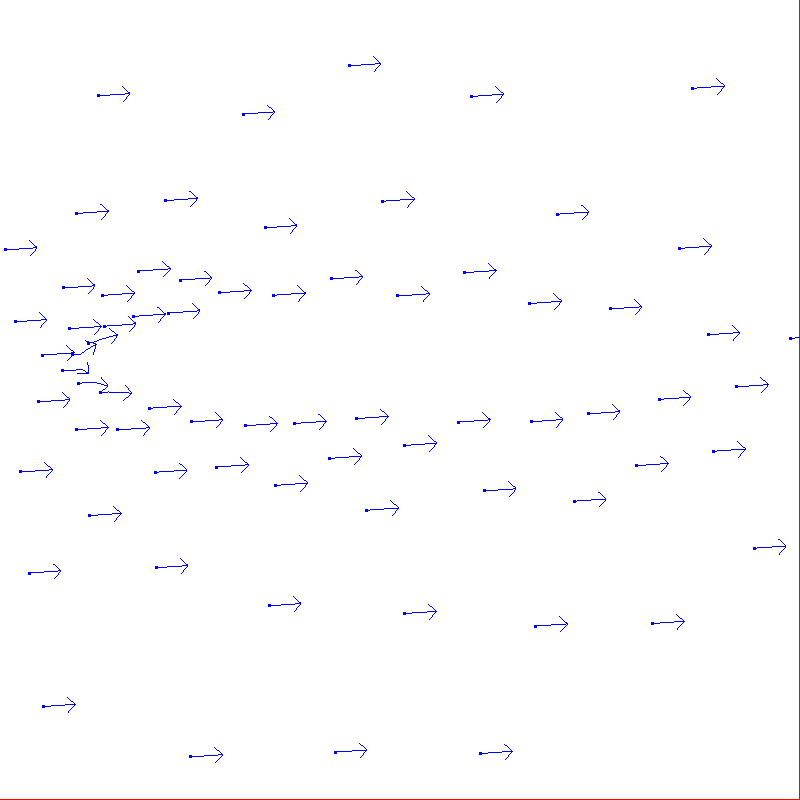
\includegraphics[width=0.8\textwidth]{jy1.png}}}
\end{minipage}
\begin{minipage}[t]{0.5\linewidth}
\subfigure{\label{1.2}}
\addtocounter{subfigure}{-2}
\subfigure[]{\subfigure{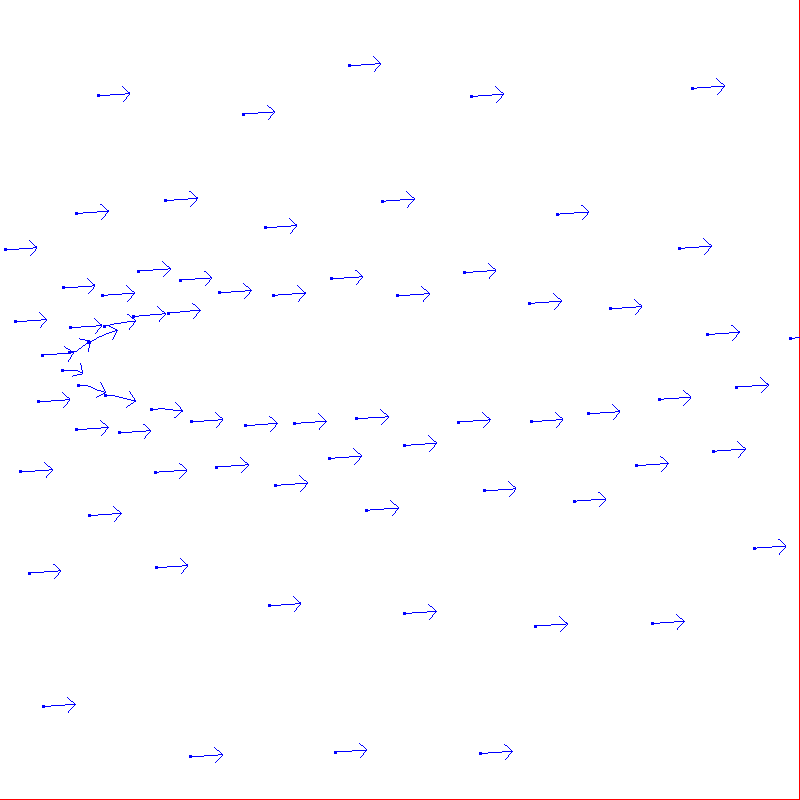
\includegraphics[width=0.8\textwidth]{jy3.png}}}
\end{minipage}
\begin{minipage}[t]{0.5\linewidth}
\subfigure{\label{1.3}}
\addtocounter{subfigure}{-2}
\subfigure[]{\subfigure{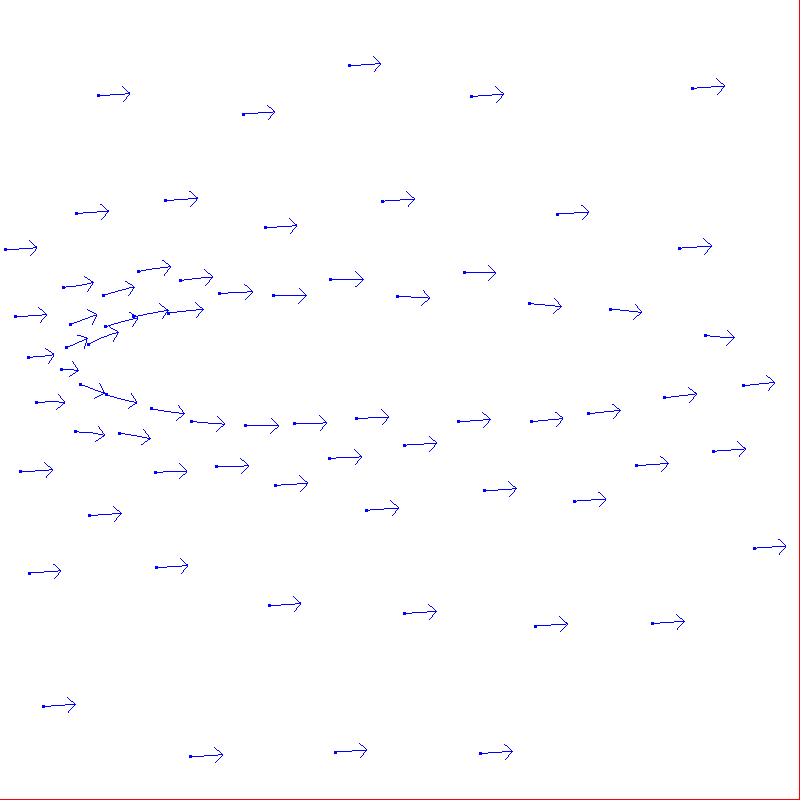
\includegraphics[width=0.8\textwidth]{jy5.png}}}
\end{minipage}
\begin{minipage}[t]{0.5\linewidth}
\subfigure{\label{1.4}}
\addtocounter{subfigure}{-2}
\subfigure[]{\subfigure{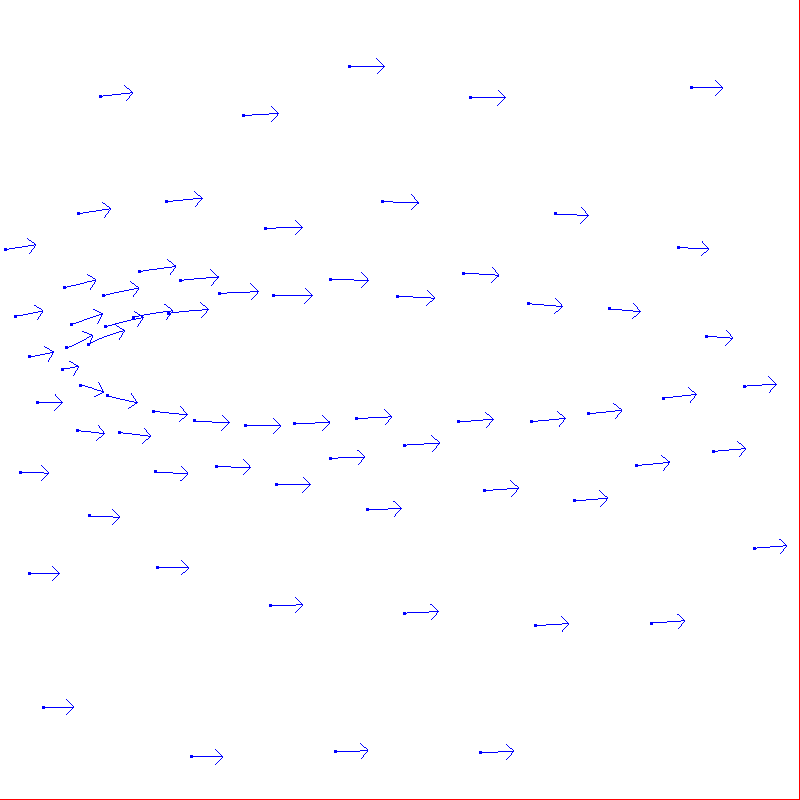
\includegraphics[width=0.8\textwidth]{jy7.png}}}
\end{minipage}
\begin{minipage}[t]{0.5\linewidth}
\subfigure{\label{1.5}}
\addtocounter{subfigure}{-2}
\subfigure[]{\subfigure{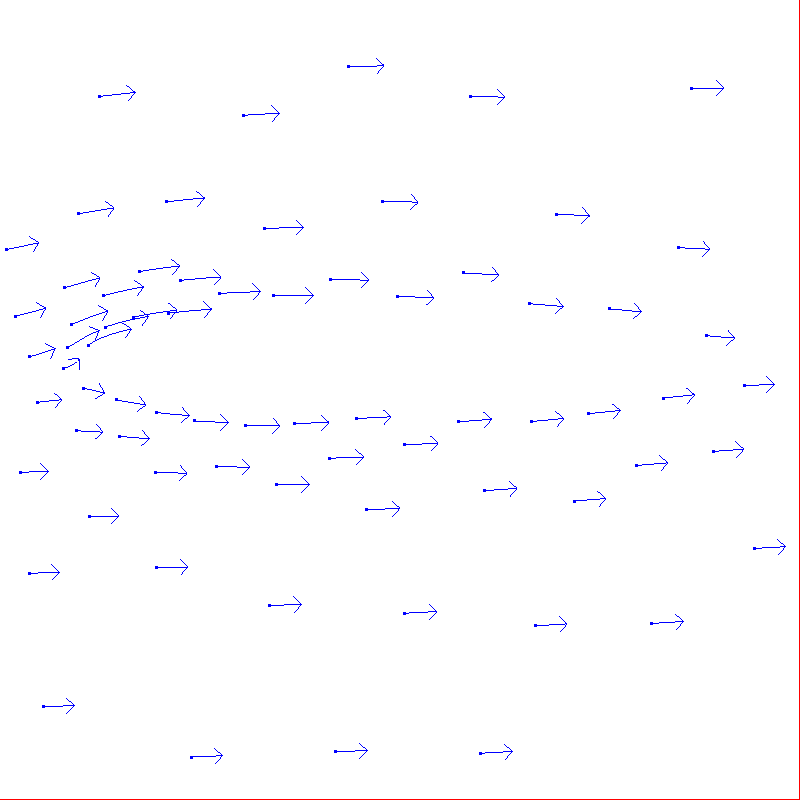
\includegraphics[width=0.8\textwidth]{jy9.png}}}
\end{minipage}
\begin{minipage}[t]{0.5\linewidth}
\subfigure{\label{1.6}}
\addtocounter{subfigure}{-2}
\subfigure[]{\subfigure{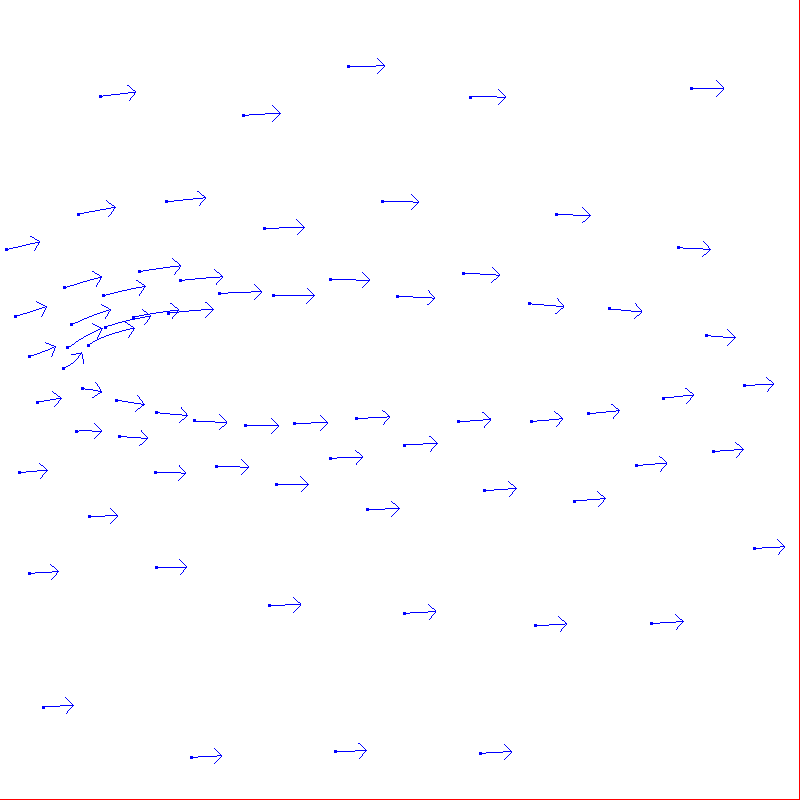
\includegraphics[width=0.8\textwidth]{jy11.png}}}
\end{minipage}
\caption{Speed field around an airfoil}
\end{figure}
\end{center}
\newpage
\indent This series of figures present the flow field around a airfoil in 2-D.It is clear that as time passing by,the speed of air above the airfoil increases fast,while the speed decreases a little,beneath.\\
\indent However,it is dangerous to use the same distance function and the same visualization strategy despite the differences.Definitely,using the appropriate strategy helps emphasizing the characteristic,while unsuitable ones cover it.Here is an example.For the same flow field,different distance function and different visualization strategy are used,resulting enormous differences between these tow series of figures.\\
\indent In the first group of figures (fig.\ref{2}),we use $E(x)=\int_{V_i}\frac{d^2(x,s)}{F(s)}ds$ as the energy function.So that the CVT generators gather to where the speed is low.And we simply draw the vectors without modify.As a result,the two vortices is not apparent in the first group.However,in the second group (fig.\ref{2}),the energy function is as normal but we draw the vectors with the length reciprocal and streamlined,to prominent the vortices.\\

\begin{center}
\begin{figure}[htbp]
\centering
\begin{minipage}[t]{0.4\linewidth}
\subfigure{\label{2.1}}
\addtocounter{subfigure}{-2}
\subfigure[]{\subfigure{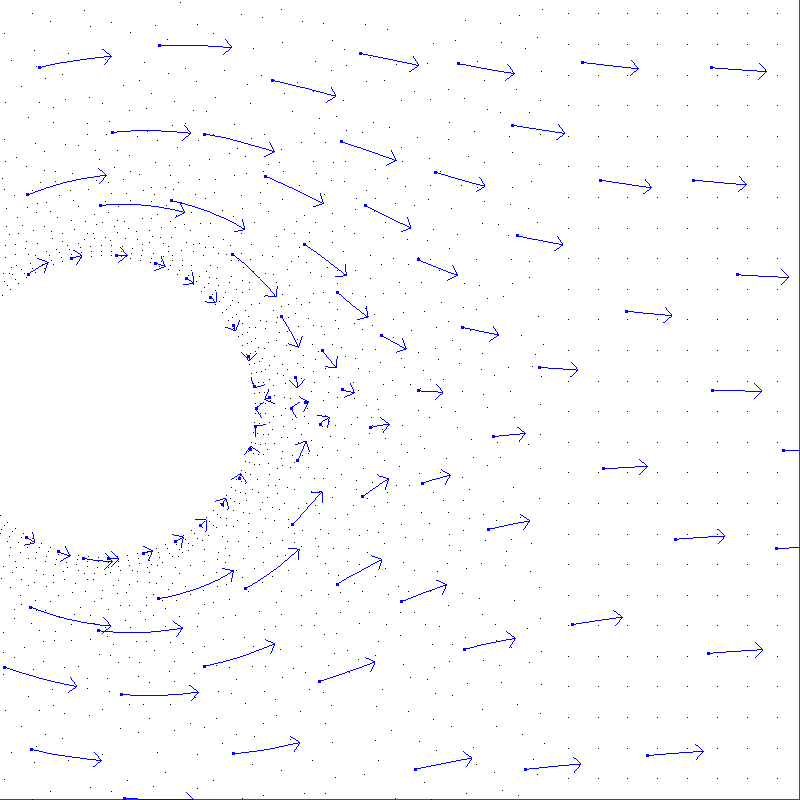
\includegraphics[width=1\textwidth]{smallarrow1.png}}}
\end{minipage}
\begin{minipage}[t]{0.4\linewidth}
\subfigure{\label{2.2}}
\addtocounter{subfigure}{-2}
\subfigure[]{\subfigure{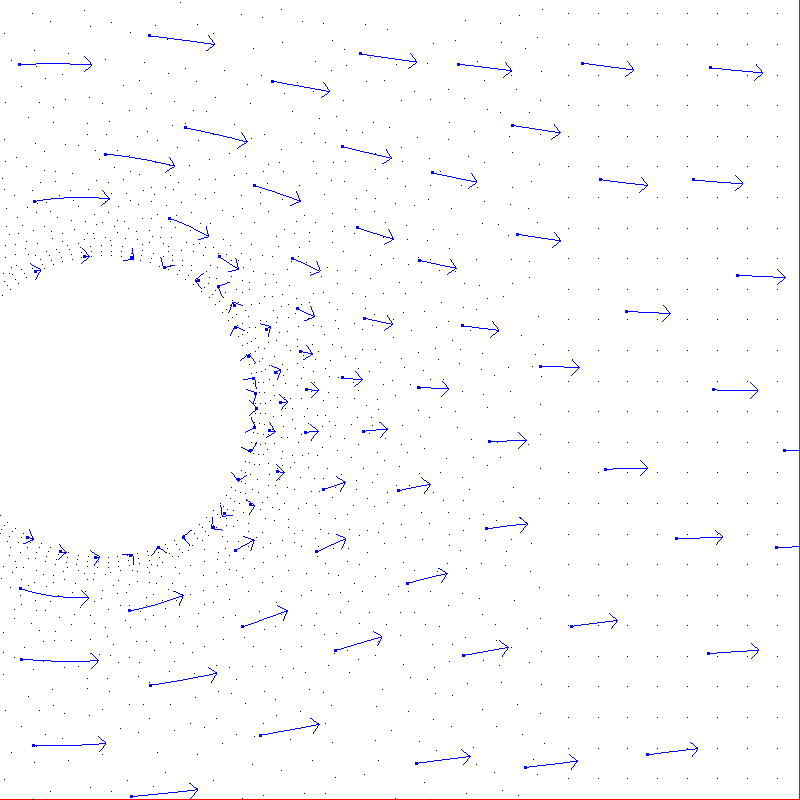
\includegraphics[width=1\textwidth]{smallarrow2.png}}}
\end{minipage}
\begin{minipage}[t]{0.4\linewidth}
\subfigure{\label{2.3}}
\addtocounter{subfigure}{-2}
\subfigure[]{\subfigure{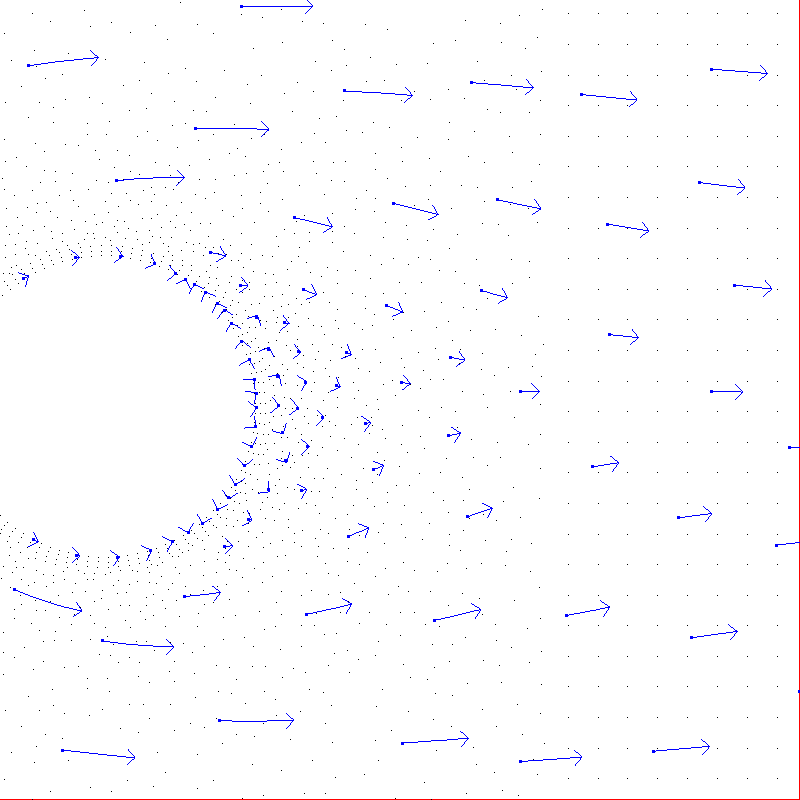
\includegraphics[width=1\textwidth]{smallarrow3.png}}}
\end{minipage}
\begin{minipage}[t]{0.4\linewidth}
\subfigure{\label{2.4}}
\addtocounter{subfigure}{-2}
\subfigure[]{\subfigure{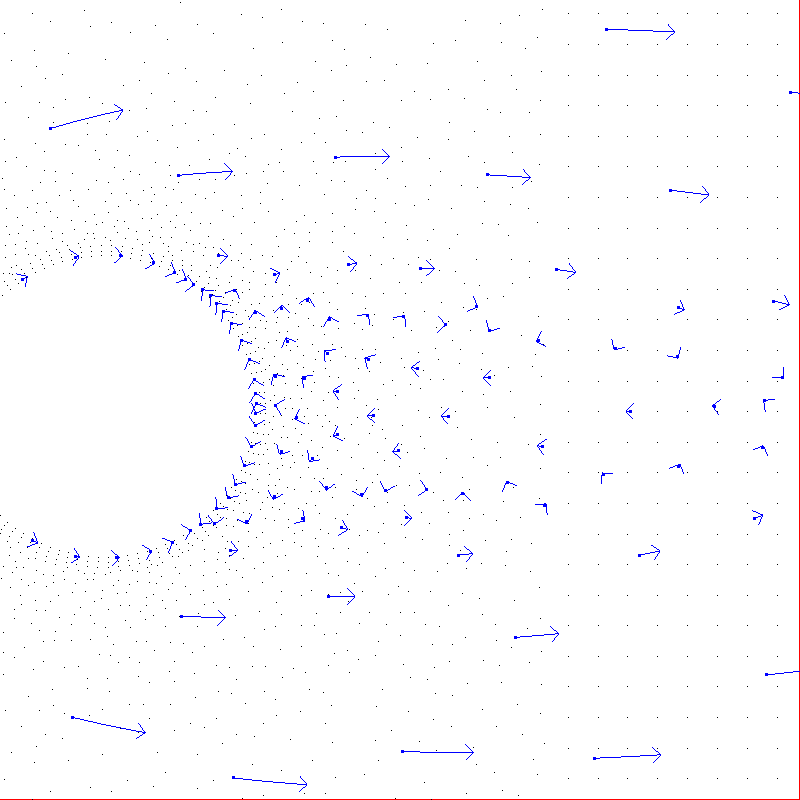
\includegraphics[width=1\textwidth]{smallarrow4.png}}}
\end{minipage}
\begin{minipage}[t]{0.4\linewidth}
\subfigure{\label{2.5}}
\addtocounter{subfigure}{-2}
\subfigure[]{\subfigure{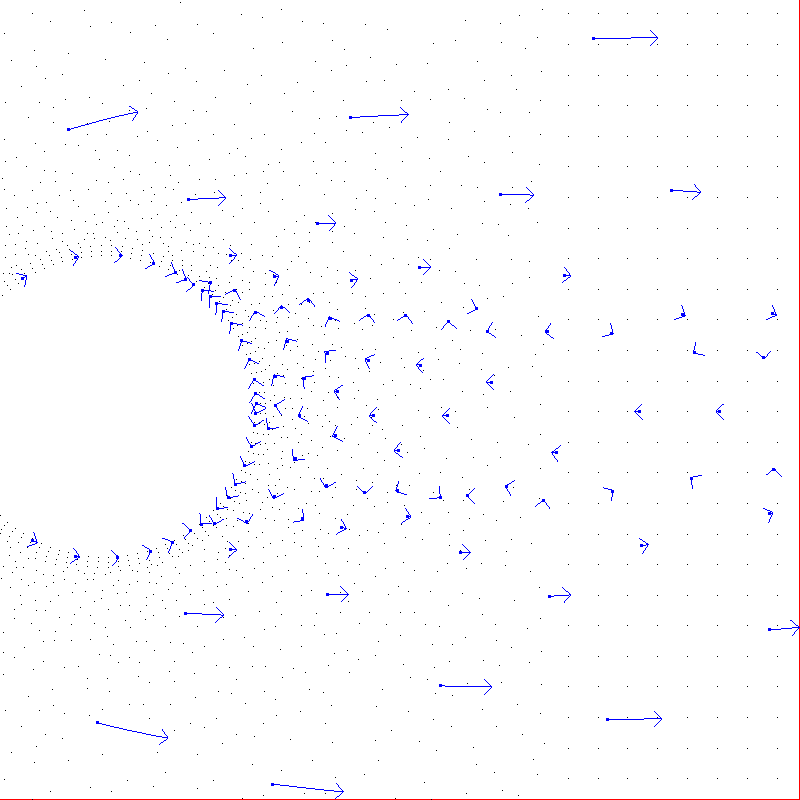
\includegraphics[width=1\textwidth]{smallarrow5.png}}}
\end{minipage}
\begin{minipage}[t]{0.4\linewidth}
\subfigure{\label{2.6}}
\addtocounter{subfigure}{-2}
\subfigure[]{\subfigure{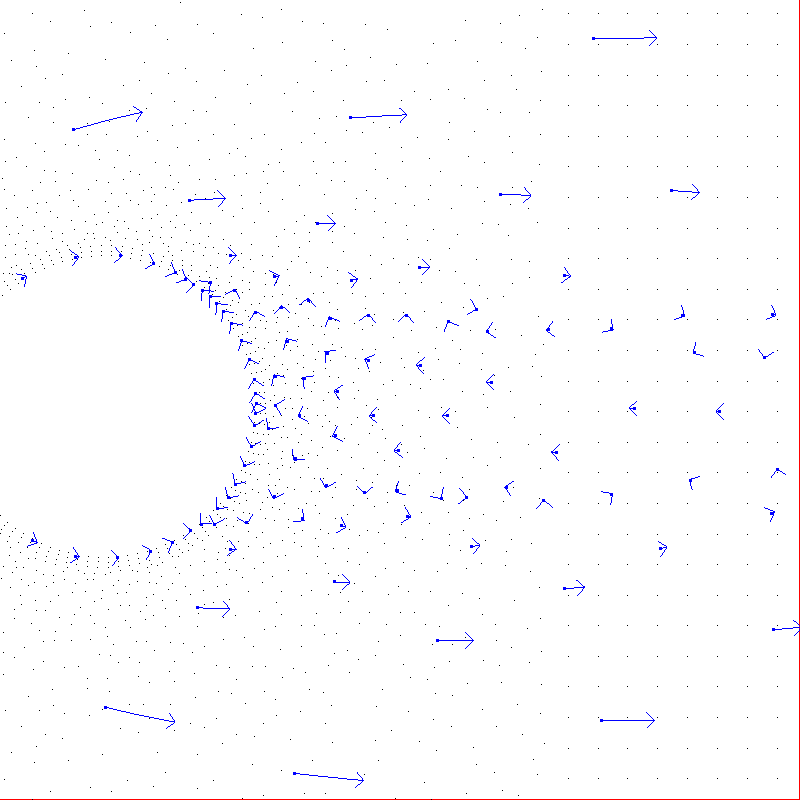
\includegraphics[width=1\textwidth]{smallarrow6.png}}}
\end{minipage}
\caption{Liquid around a pile,first}
\label{2}
\end{figure}
\end{center}

\begin{center}
\begin{figure}[htbp]
\centering
\begin{minipage}[t]{0.4\linewidth}
\subfigure{\label{3.1}}
\addtocounter{subfigure}{-2}
\subfigure[]{\subfigure{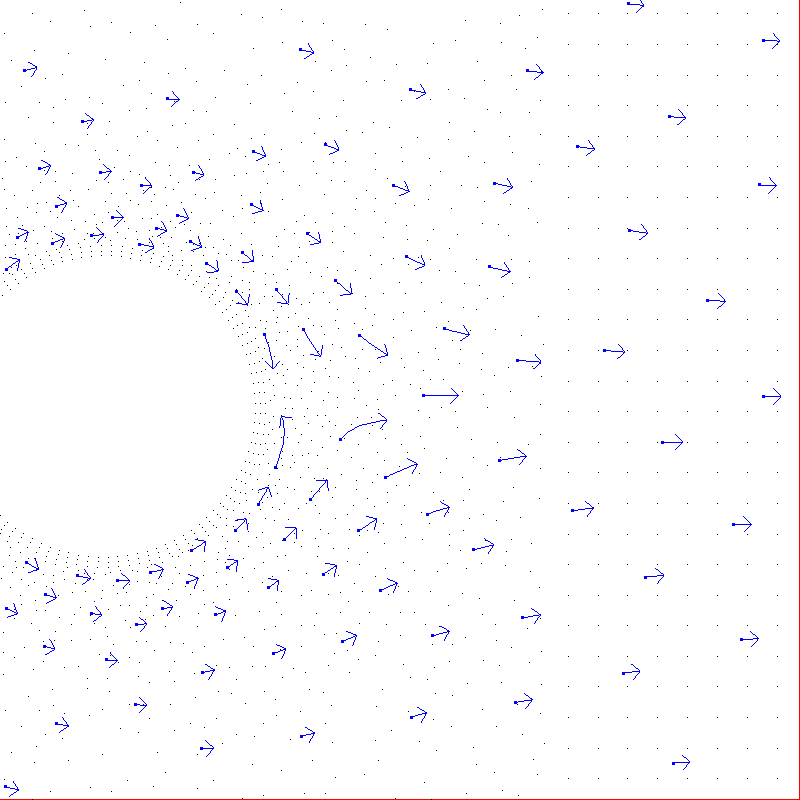
\includegraphics[width=1\textwidth]{bigarrow1.png}}}
\end{minipage}
\begin{minipage}[t]{0.4\linewidth}
\subfigure{\label{3.2}}
\addtocounter{subfigure}{-2}
\subfigure[]{\subfigure{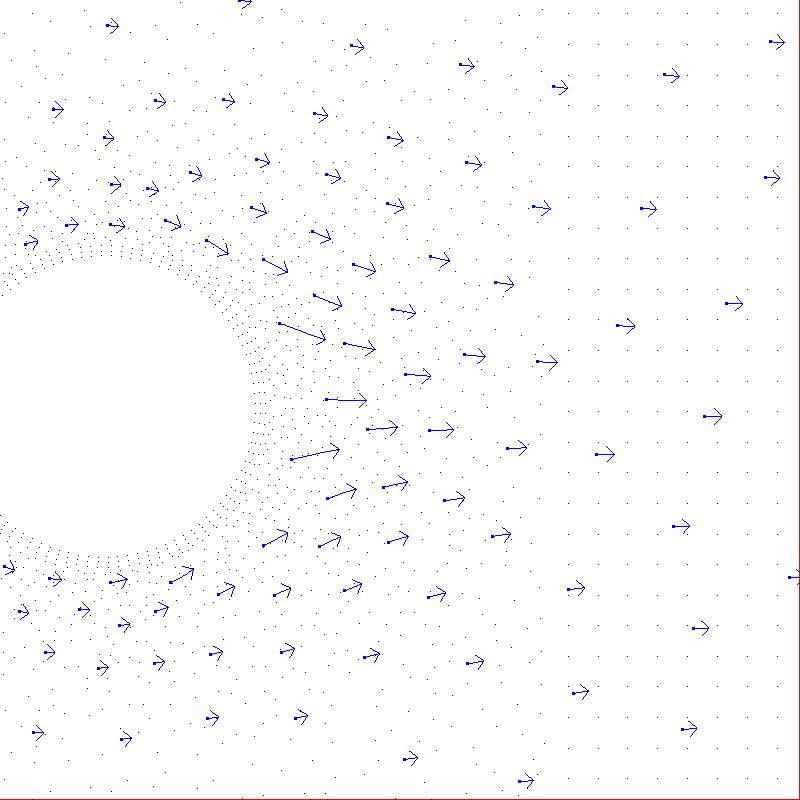
\includegraphics[width=1\textwidth]{bigarrow2.png}}}
\end{minipage}
\begin{minipage}[t]{0.4\linewidth}
\subfigure{\label{3.3}}
\addtocounter{subfigure}{-2}
\subfigure[]{\subfigure{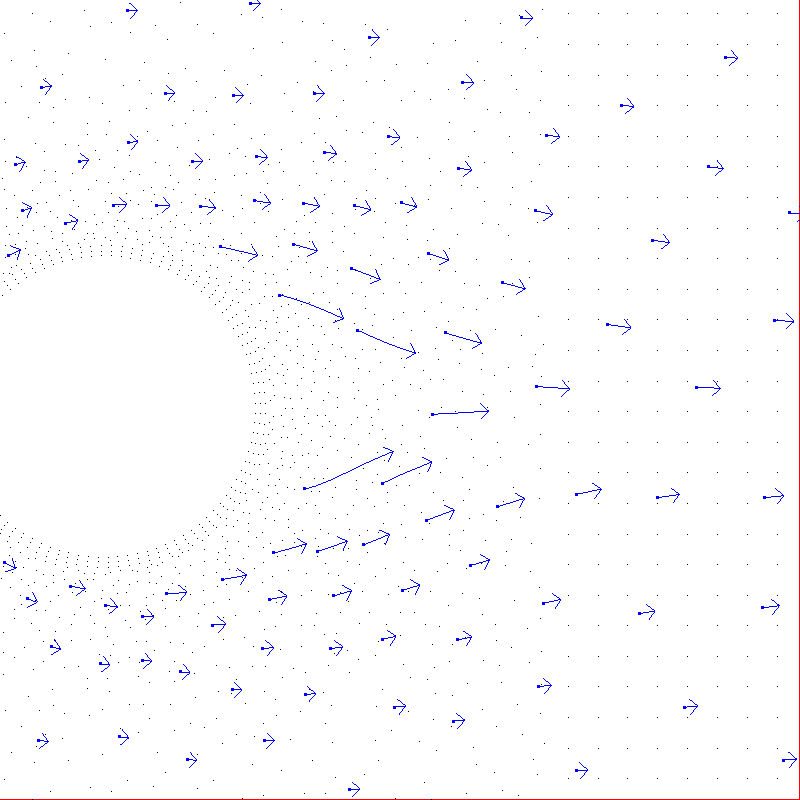
\includegraphics[width=1\textwidth]{bigarrow3.png}}}
\end{minipage}
\begin{minipage}[t]{0.4\linewidth}
\subfigure{\label{3.4}}
\addtocounter{subfigure}{-2}
\subfigure[]{\subfigure{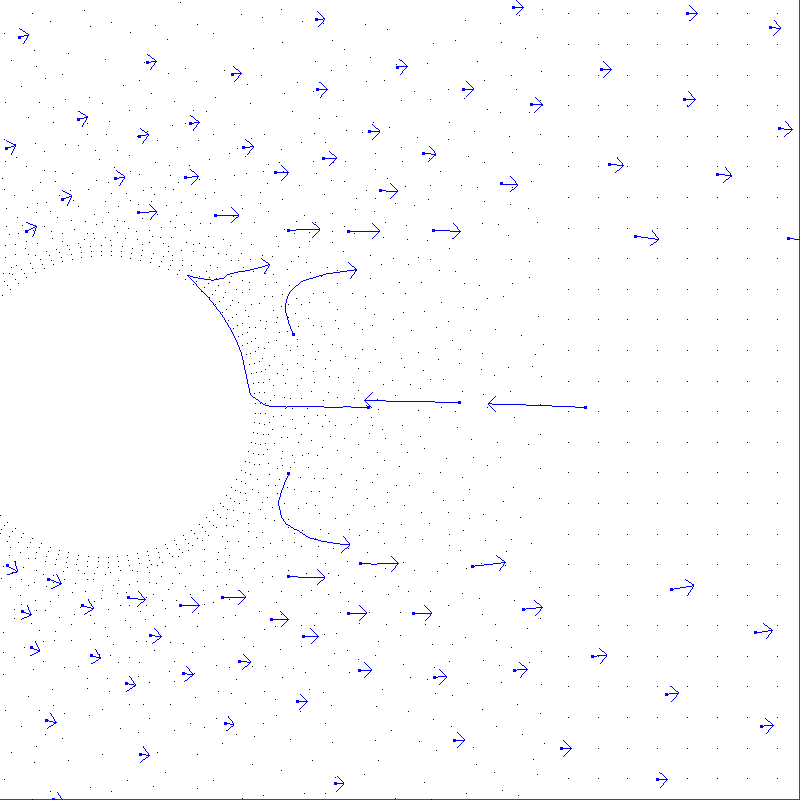
\includegraphics[width=1\textwidth]{bigarrow4.png}}}
\end{minipage}
\begin{minipage}[t]{0.4\linewidth}
\subfigure{\label{3.5}}
\addtocounter{subfigure}{-2}
\subfigure[]{\subfigure{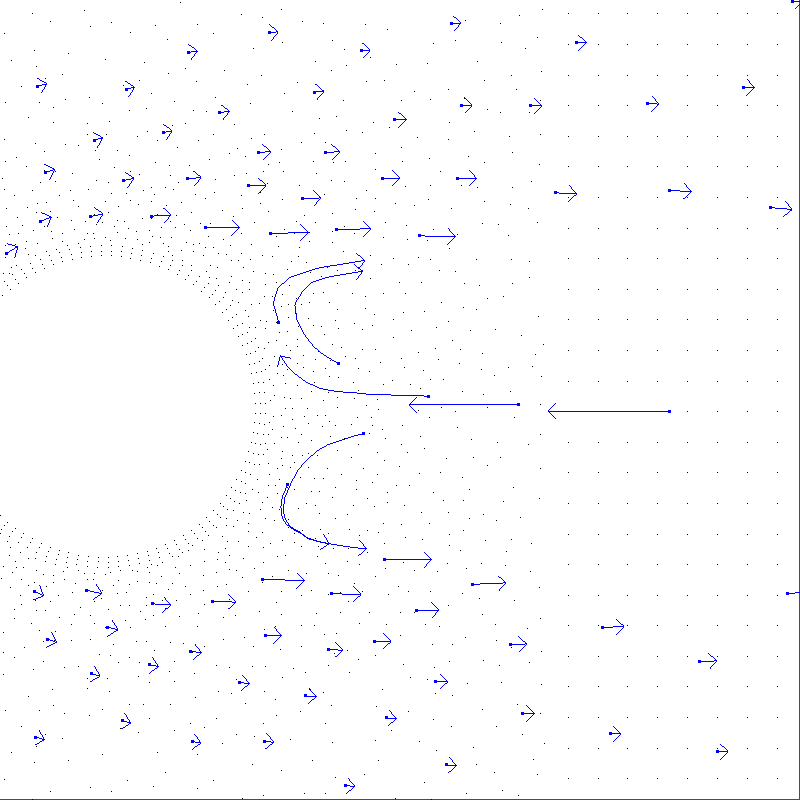
\includegraphics[width=1\textwidth]{bigarrow5.png}}}
\end{minipage}
\begin{minipage}[t]{0.4\linewidth}
\subfigure{\label{3.6}}
\addtocounter{subfigure}{-2}
\subfigure[]{\subfigure{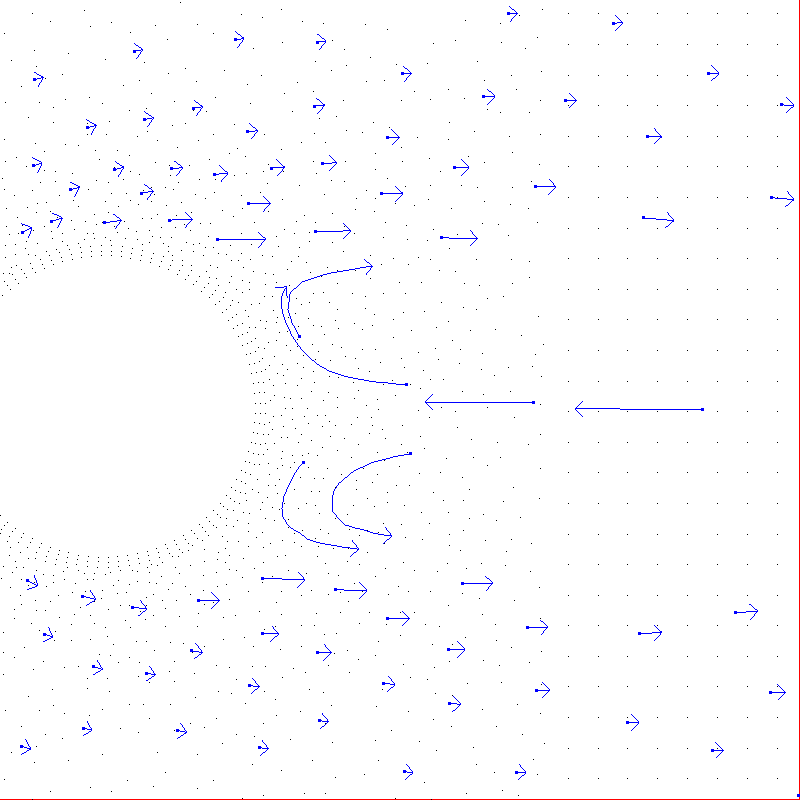
\includegraphics[width=1\textwidth]{bigarrow6.png}}}
\end{minipage}
\caption{Liquid around a pile,second}
\label{3}
\end{figure}
\end{center}


% An example of a floating figure using the graphicx package.
% Note that \label must occur AFTER (or within) \caption.
% For figures, \caption should occur after the \includegraphics.
% Note that IEEEtran v1.7 and later has special internal code that
% is designed to preserve the operation of \label within \caption
% even when the captionsoff option is in effect. However, because
% of issues like this, it may be the safest practice to put all your
% \label just after \caption rather than within \caption{}.
%
% Reminder: the "draftcls" or "draftclsnofoot", not "draft", class
% option should be used if it is desired that the figures are to be
% displayed while in draft mode.
%
%\begin{figure}[!t]
%\centering
%\includegraphics[width=2.5in]{myfigure}
% where an .eps filename suffix will be assumed under latex,
% and a .pdf suffix will be assumed for pdflatex; or what has been declared
% via \DeclareGraphicsExtensions.
%\caption{Simulation results for the network.}
%\label{fig_sim}
%\end{figure}

% Note that the IEEE typically puts floats only at the top, even when this
% results in a large percentage of a column being occupied by floats.
% However, the Computer Society has been known to put floats at the bottom.


% An example of a double column floating figure using two subfigures.
% (The subfig.sty package must be loaded for this to work.)
% The subfigure \label commands are set within each subfloat command,
% and the \label for the overall figure must come after \caption.
% \hfil is used as a separator to get equal spacing.
% Watch out that the combined width of all the subfigures on a
% line do not exceed the text width or a line break will occur.
%
%\begin{figure*}[!t]
%\centering
%\subfloat[Case I]{\includegraphics[width=2.5in]{box}%
%\label{fig_first_case}}
%\hfil
%\subfloat[Case II]{\includegraphics[width=2.5in]{box}%
%\label{fig_second_case}}
%\caption{Simulation results for the network.}
%\label{fig_sim}
%\end{figure*}
%
% Note that often IEEE papers with subfigures do not employ subfigure
% captions (using the optional argument to \subfloat[]), but instead will
% reference/describe all of them (a), (b), etc., within the main caption.
% Be aware that for subfig.sty to generate the (a), (b), etc., subfigure
% labels, the optional argument to \subfloat must be present. If a
% subcaption is not desired, just leave its contents blank,
% e.g., \subfloat[].


% An example of a floating table. Note that, for IEEE style tables, the
% \caption command should come BEFORE the table and, given that table
% captions serve much like titles, are usually capitalized except for words
% such as a, an, and, as, at, but, by, for, in, nor, of, on, or, the, to
% and up, which are usually not capitalized unless they are the first or
% last word of the caption. Table text will default to \footnotesize as
% the IEEE normally uses this smaller font for tables.
% The \label must come after \caption as always.
%
%\begin{table}[!t]
%% increase table row spacing, adjust to taste
%\renewcommand{\arraystretch}{1.3}
% if using array.sty, it might be a good idea to tweak the value of
% \extrarowheight as needed to properly center the text within the cells
%\caption{An Example of a Table}
%\label{table_example}
%\centering
%% Some packages, such as MDW tools, offer better commands for making tables
%% than the plain LaTeX2e tabular which is used here.
%\begin{tabular}{|c||c|}
%\hline
%One & Two\\
%\hline
%Three & Four\\
%\hline
%\end{tabular}
%\end{table}


% Note that the IEEE does not put floats in the very first column
% - or typically anywhere on the first page for that matter. Also,
% in-text middle ("here") positioning is typically not used, but it
% is allowed and encouraged for Computer Society conferences (but
% not Computer Society journals). Most IEEE journals/conferences use
% top floats exclusively.
% Note that, LaTeX2e, unlike IEEE journals/conferences, places
% footnotes above bottom floats. This can be corrected via the
% \fnbelowfloat command of the stfloats package.



\newpage
\section{Conclusion}
\indent We have improve the CVT visualization by using the short streamline and inheriting the generators.The short streamline express more direction information of the vector field.The inheriting of generators reduces the time cost of calculation as well as show the change of fields more clearly.By this two mean,it is able to visualization the flow field more representative.\\
\indent Comparing to other visualization method,CVT visualization has the advantage as global-visualized, accessable, efficient, adjustable.While other visualization methods,called filters, are likely to choose some of the origin points to render,the CVT visualization is to generate the points for rendering.This enable us to demonstrate the key point and ignore the useless part of the data.Therefore,we can generate the key points and highlight the characteristic.\\
\indent However,there are still some problem existing.It is obvious that the final CVT is only determined by the choice of initial generators as long as the distance function does not change.But there is not any theory about how to choose the seed in the first iteration.Since the CVT is merely a local minimum of energy function,it is likely that different seeds choosing result extraordinary distinct CVT.Also,if there is an uniform strategy for visualization,it would be able to save a lot of time try different visualization strategy.These questions are worthy of further study.





% if have a single appendix:
%\appendix[Proof of the Zonklar Equations]
% or
%\appendix  % for no appendix heading
% do not use \section anymore after \appendix, only \section*
% is possibly needed

% use appendices with more than one appendix
% then use \section to start each appendix
% you must declare a \section before using any
% \subsection or using \label (\appendices by itself
% starts a section numbered zero.)
%


%\appendices
%\section{Proof of the First Zonklar Equation}
%Appendix one text goes here.

% you can choose not to have a title for an appendix
% if you want by leaving the argument blank
%\section{}
%Appendix two text goes here.


% use section* for acknowledgment
%\ifCLASSOPTIONcompsoc
  % The Computer Society usually uses the plural form
  %\section*{Acknowledgments}
%\else
  % regular IEEE prefers the singular form
  %\section*{Acknowledgment}
%\fi


%The authors would like to thank...


% Can use something like this to put references on a page
% by themselves when using endfloat and the captionsoff option.
\ifCLASSOPTIONcaptionsoff
  \newpage
\fi



% trigger a \newpage just before the given reference
% number - used to balance the columns on the last page
% adjust value as needed - may need to be readjusted if
% the document is modified later
%\IEEEtriggeratref{8}
% The "triggered" command can be changed if desired:
%\IEEEtriggercmd{\enlargethispage{-5in}}

% references section

% can use a bibliography generated by BibTeX as a .bbl file
% BibTeX documentation can be easily obtained at:
% http://mirror.ctan.org/biblio/bibtex/contrib/doc/
% The IEEEtran BibTeX style support page is at:
% http://www.michaelshell.org/tex/ieeetran/bibtex/
%\bibliographystyle{IEEEtran}
% argument is your BibTeX string definitions and bibliography database(s)
%\bibliography{IEEEabrv,../bib/paper}
%
% <OR> manually copy in the resultant .bbl file
% set second argument of \begin to the number of references
% (used to reserve space for the reference number labels box)
\begin{thebibliography}{1}

\bibitem{IEEEhowto:kopka}
H.~Kopka and P.~W. Daly, \emph{A Guide to {\LaTeX}}, 3rd~ed.\hskip 1em plus
  0.5em minus 0.4em\relax Harlow, England: Addison-Wesley, 1999.
\bibitem{1}
Du Q, Wang X. Centroidal Voronoi tessellation based algorithms for vector fields visualization and segmentation[C]// Visualization. IEEE, 2004:43-50.
\bibitem{2}
Du Q, Wang D. Anisotropic centroidal Voronoi tessellations and their applications[J]. Siam Journal on Scientific Computing, 2005, 26(3):737--761.
\bibitem{3}
Hateley J C, Wei H, Chen L. Fast Methods for Computing Centroidal Voronoi Tessellations[J]. Journal of Scientific Computing, 2014, 63(1):185-212.
\bibitem{4}
DU, Q., AND WANG, X. 2004. Tessellation and clustering by mixture
models and their parallel implementations. In Proceedings
of the 2004 SIAM data mining conference, Orlando, FL, SIAM.
\end{thebibliography}
% biography section
%
% If you have an EPS/PDF photo (graphicx package needed) extra braces are
% needed around the contents of the optional argument to biography to prevent
% the LaTeX parser from getting confused when it sees the complicated
% \includegraphics command within an optional argument. (You could create
% your own custom macro containing the \includegraphics command to make things
% simpler here.)
%\begin{IEEEbiography}[{\includegraphics[width=1in,height=1.25in,clip,keepaspectratio]{mshell}}]{Michael Shell}
% or if you just want to reserve a space for a photo:

%\begin{IEEEbiography}{Michael Shell}
%Biography text here.
%\end{IEEEbiography}

% if you will not have a photo at all:
%\begin{IEEEbiographynophoto}{John Doe}
%Biography text here.
%\end{IEEEbiographynophoto}

% insert where needed to balance the two columns on the last page with
% biographies
%\newpage

%\begin{IEEEbiographynophoto}{Jane Doe}
%Biography text here.
%\end{IEEEbiographynophoto}

% You can push biographies down or up by placing
% a \vfill before or after them. The appropriate
% use of \vfill depends on what kind of text is
% on the last page and whether or not the columns
% are being equalized.

%\vfill

% Can be used to pull up biographies so that the bottom of the last one
% is flush with the other column.
%\enlargethispage{-5in}



% that's all folks
\end{document}


